%%%%%%%Pour le handout
% \documentclass[xcolor=dvipsnames,table]{article}
% \usepackage{beamerarticle}
% \usepackage{fullpage}
% \linespread{1.3}
%\usepackage{tlingmacros}

%%%%%%%Pour la présentation
\documentclass[utf8x]{beamer}
\usepackage{etex}
\usepackage[T1]{fontenc}
\usepackage[french]{babel}
\usepackage{ucs}
%\usepackage[latin1]{inputenc}


\usepackage{amssymb}
\usepackage{amsmath}
%\setcounter{tocdepth}{3}
\usepackage{graphicx}
\usepackage{mathrsfs}
\usepackage{multirow}
\usepackage{multicol,longtable,booktabs} %% pour des tableaux plus compliquées           
\usepackage{url}
\usepackage{xspace}
\usepackage{graphicx}
\usepackage{theorem}
\usepackage{fourier}
\usepackage{tipa}
\usepackage{color}
\usepackage{colortbl}
\usepackage{GJ}
\usepackage{walther-pres-en}
\usepackage{graphicx}
\usepackage{eurosym}
\usepackage{slashbox,pict2e}

\usepackage{array}
\newcolumntype{L}[1]{>{\raggedright\let\newline\\\arraybackslash\hspace{0pt}}m{#1}}
\newcolumntype{C}[1]{>{\centering\let\newline\\\arraybackslash\hspace{0pt}}m{#1}}
\newcolumntype{R}[1]{>{\raggedleft\let\newline\\\arraybackslash\hspace{0pt}}m{#1}}

\usepackage{linguex}

\usepackage{subfigure}
\usepackage{wrapfig}
%%%%tikz
%\usepackage[usenames,dvipsnames]{xcolor}
\usepackage{tikz}
\usetikzlibrary{arrows,automata,positioning}

\tikzset{
    state/.style={
           rectangle,
           rounded corners,
           draw=black, very thick,
           minimum height=2em,
           inner sep=2pt,
           text centered,
           },
}

\usepackage{pgfplots}
\usepackage{pgfplotstable}





% \newlength{\btarrowsize} 
% \pgfarrowsdeclare{biggertip}{biggertip}{ 
%  \setlength{\btarrowsize}{0.4pt} 
%  \addtolength{\btarrowsize}{.5\pgflinewidth} 
%  \pgfarrowsrightextend{0} 
%  \pgfarrowsleftextend{-5\btarrowsize} 
% }{ 
%  \setlength{\btarrowsize}{0.4pt} 
%  \addtolength{\btarrowsize}{.5\pgflinewidth} 
%  \pgfpathmoveto{\pgfpoint{-5\btarrowsize}{4\btarrowsize}} 
%  \pgfpathlineto{\pgfpointorigin} 
%  \pgfpathlineto{\pgfpoint{-5\btarrowsize}{-4\btarrowsize}} 
%  \pgfusepathqstroke 
% }
%pour le fichier de translittération:
% \usepackage{fontspec}
% \usepackage{xCJK}
% \usepackage[overlap,CJK]{ruby}	  % Furigana support
% \renewcommand{\rubysize}{0.5}	  % Furigana size
% \renewcommand{\rubysep}{-0.3ex}	  % Spacing between Furigana and Kanji
% \setCJKmainfont{STSong}
% \setCJKfamilyfont{latin}{Times}
% \usepackage{xCJK}


%%%%%%%%%

\newcommand{\twocolumnblocks}[6]{
\begin{columns}[onlytextwidth]
\begin{column}{.48\textwidth}\begin{#1}{#2}#3\end{#1}\end{column}
\begin{column}{.48\textwidth}\begin{#4}{#5}#6\end{#4}\end{column}
\end{columns}
}

\newenvironment{blackwideitemize}{\itemize\addtolength{\itemsep}{6pt}}{\enditemize}
\newenvironment{wideitemize}{\color{dodgerblue4}\itemize\addtolength{\itemsep}{6pt}}{\enditemize}
%\newenvironment{wideitemize}{\itemize}{\enditemize}
\newenvironment{smallwideitemize}{\color{gray11}\small\itemize\addtolength{\itemsep}{4pt}}{\enditemize}
%\newenvironment{wideitemize}{\itemize}{\enditemize}

\newcolumntype{x}[1]{%
>{\raggedright\arraybackslash\hspace{0pt}}p{#1}}%


%%%bullets:\item<green@1-> A pro item
\newenvironment{greenenv}{\only{\setbeamercolor{local structure}{fg=green}}}{}
\newenvironment{orangeenv}{\only{\setbeamercolor{local structure}{fg=orange}}}{}
\newenvironment{redenv}{\only{\setbeamercolor{local structure}{fg=red}}}{}
\newenvironment{magentaenv}{\only{\setbeamercolor{local
      structure}{fg=red}}}{}
\newenvironment{blueenv}{\only{\setbeamercolor{local structure}{fg=blue}}}{}
\newenvironment{cyanenv}{\only{\setbeamercolor{local
      structure}{fg=cyan}}}{}

%%The following code defines the macros \dotuline and \dashuline:
\usepackage[normalem]{ulem}
\def\dotuline{\bgroup
  \ifdim\ULdepth=\maxdimen  % Set depth based on font, if not set already
   \settodepth\ULdepth{(j}\advance\ULdepth.4pt\fi
  \markoverwith{\begingroup
  \advance\ULdepth0.08ex
  \lower\ULdepth\hbox{\kern.15em .\kern.1em}%
  \endgroup}\ULon}

\def\dashuline{\bgroup
  \ifdim\ULdepth=\maxdimen  % Set depth based on font, if not set already
   \settodepth\ULdepth{(j}\advance\ULdepth.4pt\fi
  \markoverwith{\kern.15em
  \vtop{\kern\ULdepth \hrule width .3em}%
  \kern.15em}\ULon}
  
%  \NoAutoSpaceBeforeFDP % utile pour les citations avec :
% - - - - - - - - - - - - - - - - - - - - - - - - - - - - - - - - - - - - - - -
%\usetheme{Boadilla}
\usetheme{CambridgeUS}
%\usetheme{Singapore}
%\usetheme{Berlin}
%\usetheme{AnnArbor}
\usecolortheme{seagull}
%\usecolortheme{crane}
%\usecolortheme{dove}
%\usecolortheme[0.91,0.59,0.48]{dove}
%\usefonttheme{professionalfonts}
%\usecolortheme[RGB={100,175,5}]{structure}
%\usecolortheme[RGB={0.91,0.59,0.48}]{structure}
\setbeamertemplate{navigation symbols}{}
%\setbeamertemplate{items}[circle]
\setbeamertemplate{blocks}[rounded]
% Avoid total frame number
\makeatletter
\setbeamertemplate{footline}
{
  \leavevmode%
  \hbox{%
  \begin{beamercolorbox}[wd=.39\paperwidth,ht=2.25ex,dp=1ex,center]{author in head/foot}%
    \usebeamerfont{author in head/foot}\insertshortauthor~~\beamer@ifempty{\insertshortinstitute}{}{(\insertshortinstitute)}
  \end{beamercolorbox}%
  \begin{beamercolorbox}[wd=.34\paperwidth,ht=2.25ex,dp=1ex,center]{title in head/foot}%
    \usebeamerfont{title in head/foot}\insertshorttitle
  \end{beamercolorbox}%
  \begin{beamercolorbox}[wd=.28\paperwidth,ht=2.25ex,dp=1ex,right]{date in head/foot}%
    \usebeamerfont{date in head/foot}\insertshortdate{}\hspace*{2em}
    \insertframenumber / \inserttotalframenumber\hspace*{2ex} 
  \end{beamercolorbox}}%
  \vskip0pt%
}
\makeatother

\usefonttheme[stillsansseriftext]{serif}

\setbeamercolor{normal text}{fg=gray11}
\setbeamerfont{frametitle}{%
  family=\rmfamily,font=sans}
\setbeamerfont{section number projected}{%
  family=\rmfamily,size=\small}
\setbeamercolor{section number
  projected}{bg=lightsteelblue1,fg=midnightblue}
\setbeamercolor{title}{fg=midnightblue}
\setbeamercolor{title}{bg=white}
\setbeamercolor{subtitle}{fg=slategray4}
\setbeamercolor{author}{fg=dodgerblue4}
\setbeamercolor{institute}{fg=slategrey}
\setbeamercolor{date}{fg=slategrey}
\setbeamercolor{frametitle}{fg=midnightblue}
\setbeamercolor{frametitle}{bg=gray91}
\setbeamercolor{structure}{fg=dodgerblue4}
\setbeamercolor{postit}{fg=midnightblue,bg=ghostwhite!20!ghostwhite} % - - - - - - - - - - - - - - - - - - - - - - - - - - - - - - - - - - - - - - -
%\iffalse
\AtBeginSection[]
{
\begin{frame}[noframenumbering]
       \frametitle{\darkhighlightiii{Outline}}
       \tableofcontents[currentsubsection]
   \end{frame}
}
%\fi

\AtBeginSubsection[]
{
\begin{frame}[noframenumbering]
       \frametitle{\darkhighlightiii{Outline}}
       \tableofcontents[currentsubsection]
   \end{frame}
}

% - - Personal macros - - - - - - - - - - - - - - - - - - - - - - - - -

\usepackage{mycolors}
% \newcommand{\invisibletext}[1]{{\color{white} #1}}
% \newcommand{\highlighti}[1]{{\color{firebrick} #1}}
% \newcommand{\highlightii}[1]{{\color{forestgreen} #1}}
% \newcommand{\highlightiii}[1]{{\color{dodgerblue4} #1}}

%%%%%%%%%%%%%%%%%%%%%%%%%%%%%%%%%%%%%%%%%%%%%%%%%%%%%%%%%%%%%%%%%%%%%%%%%%%%%%%%%%%%%%
%%%%%%%%%%%%%%%%%%%%%%%%%%%%%%%%% INCLUDE %%%%%%%%%%%%%%%%%%%%%%%%%%%%%%%%%%%%%%%%%%%%%%
%%%%%%%%%%%%%%%%%%%%%%%%%%%%%%%%%%%%%%%%%%%%%%%%%%%%%%%%%%%%%%%%%%%%%%%%%%%%%%%%%%%%%%



\title[Marquage canonique du direct/inverse]{L'inverse canonique}
  \subtitle{Vers une définition typologique de l'opposition direct/inverse}

\author[Walther/Antonov/Jacques]{G\'eraldine Walther (DDL/EFL-LLF) \&
  Anton Antonov (EFL-CRLAO) \&~Guillaume
Jacques (EFL-CRLAO)}
\institute[EFL/CRLAO/LLF/DDL]{Empirical Foundations of
  Linguistics (EFL)\\% (1. Laboratoire de Linguistique Formelle (LLF)\\
% 2. Centre de Recherche Linguistique sur l'Asie Orientale (CRLAO))\\~\\
% 1.Dynamique du Language (DDL)\\
~\\
\url{geraldine.walther@univ-lyon2.fr}\\
\url{a.antonov@gmail.com}\\
\url{rgyalrongskad@gmail.com}
}%
\date[TypoUlm 14/02/2014]{TypoUlm~~~14 février 2014}

\begin{document}

%\maketitle
\begin{frame}[noframenumbering]
  \titlepage
\end{frame}
%\begin{frame}
%\tableofcontents
%\end{frame}

%\section[Measuring ling. complexity]{The task of measuring language complexity}

\section*{Introduction}
%\input{complexitymeasures}
\begin{frame}
\frametitle{\darkhighlightiii{Introduction: l'inverse canonique}}
\framesubtitle{Vers une définition typologique de l'opposition direct/inverse}
%\pause
\begin{wideitemize}
\item Le direct/inverse fait partie des types de marquages de
  l'alignement
\begin{smallwideitemize}
\item un des marquages des systèmes d'alignement hiérarchique
\item autres alignements: accusatif, ergatif, neutre, tripartite
\pause
\item le plus souvent un marquage morphologique sur le verbe
\item indexation des deux arguments pour les verbes transitifs
\item symétrie entre formes:\\ exemple: identité formelle pour les formes \textsc{1sg>3sg} et
  \textsc{3sg>1sg}\\ à un \textsc{marqueur d'inverse} près
\pause
\item phénomène typologique moins connu
\item \cite{zuniga06}
%\pause
\end{smallwideitemize}
\end{wideitemize}
\end{frame}


\begin{frame}
\frametitle{\darkhighlightiii{Introduction: l'inverse canonique}}
\framesubtitle{La distribution des types d'alignements 
  dans le monde (carte du WALS)}
\begin{center}
\vspace*{-.3cm}
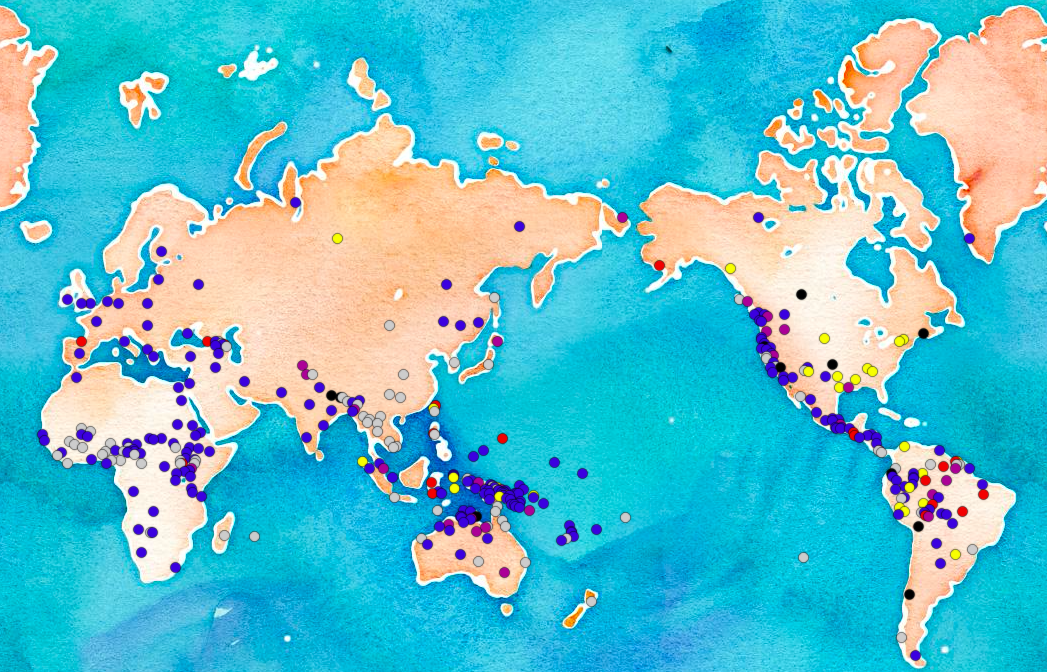
\includegraphics[width=120mm]{hierarchy}

\end{center}
\end{frame}


\begin{frame}
\frametitle{\darkhighlightiii{Introduction: l'inverse canonique}}
\framesubtitle{La distribution des langues à marquage hiérarchique
  sur le verbe (carte du WALS)}
\begin{center}
\vspace*{-.3cm}
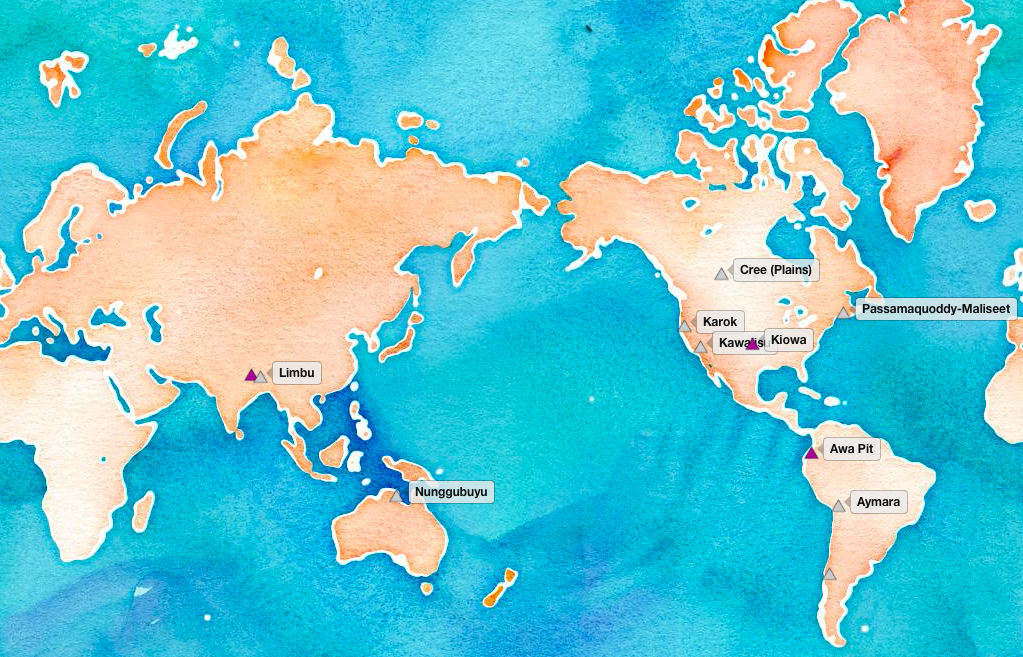
\includegraphics[width=120mm]{hierarchy-marking}

\end{center}
\end{frame}

\begin{frame}
\frametitle{\darkhighlightiii{Introduction: l'inverse canonique}}
\framesubtitle{Vers une définition typologique de l'opposition direct/inverse}
%\pause
\begin{wideitemize}
\item Un nombre non-négligeable de langues est considéré comme affichant un marquage de
  type direct/inverse
%\begin{smallwideitemize}
\item Mais la réalisation du direct/inverse varie en fait de façon
  considérable dans ces langues\\ 
\item[\highlighti{\lefthand}] Besoin d'une approche typologique du phénomène
%\end{smallwideitemize}
\end{wideitemize}
%\item But d'une approche typologique
\begin{wideitemize}
%\begin{smallwideitemize}
\item[\highlightiv{\lefthand}]~Mise en place d'un système de notions fonctionnel
\item[\highlightiv{\lefthand}] approche canonique
%\end{smallwideitemize}
\end{wideitemize}
\begin{wideitemize}
\item[\highlightii{\lefthand}] But de ce papier {\ra} proposer une définition typologiquement
  fonctionnelle des systèmes à direct/inverse
\end{wideitemize}
\end{frame}

\section[Alignement]{Les systèmes d'alignement à travers les langues}
\subsection[Alignements]{Types d'alignements à travers les langues du monde}

% a) Types d'alignements: cas idéalisés (G): ACC, ERG, NEUTRE, TRIPARTITE, HIERARCHIQUE

% \& exemples: 
% ACC - français (G); 
% ERG - basque (A); 
% NEUTRE - vietnamien (G); 
% TRIPARTITE - thulung (G); 
% HIERARCHIQUE - dargwa (G)


\begin{frame}
\frametitle{Types d'alignement}
\framesubtitle{L'alignement accusatif (cas idéalisé)}
% encodage morphologique au sein du système nominal: latin (g)


\end{frame}


\begin{frame}
\frametitle{Types d'alignement}
\framesubtitle{L'alignement accusatif (français)}
% encodage morphologique au sein du système nominal: latin (g)


\end{frame}


\begin{frame}
\frametitle{Types d'alignement}
\framesubtitle{L'alignement ergatif (cas idéalisé)}
% encodage morphologique au sein du système nominal: latin (g)


\end{frame}


\begin{frame}
\frametitle{Types d'alignement}
\framesubtitle{L'alignement ergatif (basque)}
% encodage morphologique au sein du système nominal: latin (g)


\end{frame}


\begin{frame}
\frametitle{Types d'alignement}
\framesubtitle{L'alignement neutre (cas idéalisé)}
% encodage morphologique au sein du système nominal: latin (g)


\end{frame}



\begin{frame}
\frametitle{Types d'alignement}
\framesubtitle{L'alignement neutre (vietnamien)}
% encodage morphologique au sein du système nominal: latin (g)


\end{frame}


\begin{frame}
\frametitle{Types d'alignement}
\framesubtitle{L'alignement tripartite (cas idéalisé)}
% encodage morphologique au sein du système nominal: latin (g)


\end{frame}

\begin{frame}
\frametitle{Types d'alignement}
\framesubtitle{L'alignement tripartite (thulung)}
% encodage morphologique au sein du système nominal: latin (g)


\end{frame}

\subsection[Encodage des alignements]{Encodage des alignements à travers les langues du monde}
% b) encodage des alignements (G)
% encodage syntaxique par l'ordre des mots: anglais (G)
% encodage syntaxique par des mots autonomes (préposisitons): mandarin (G)

\begin{frame}
\frametitle{Encodage syntaxique}
\framesubtitle{Ordre des mots (anglais)}
% encodage morphologique au sein du système nominal: latin (g)

\ex. Ashley love-s Bradley.\\
Ashley aimer\textsc{-3sg} Bradley\\
{\em ``Ashley aime Bradley.''}

\ex. Bradley love-s Ashley.\\
Bradley aimer\textsc{-3sg} Ashley\\
{\em ``Bradley aime Ashley.''}

\end{frame}

\begin{frame}
\frametitle{Encodage syntaxique}
\framesubtitle{Marqueurs syntaxiques (chinois mandarin)}
% encodage morphologique au sein du système nominal: latin (g)




\end{frame}


\begin{frame}
\frametitle{Encodage morphologique}
\framesubtitle{Morphologie nominale (latin)}
% encodage morphologique au sein du système nominal: latin (g)

\ex. Agricol-a lup-um vide-t.\\
paysan\textsc{(m)-nom.sg} loup\textsc{(m)-acc.sg} voir\textsc{$\backslash$\si}.-\textsc{3sg.ind.prs.act}\\
{\em ``Le paysan voit le loup.''}

\ex. Agricol-am lup-us vide-t.\\
paysan\textsc{(m)-acc.sg} loup\textsc{(m)-nom.sg} voir\textsc{$\backslash$\si}.-\textsc{3sg.ind.prs.act}\\
{\em ``Le loup voit le paysan.''}

\end{frame}

\begin{frame}
\frametitle{Encodage morphologique}
\framesubtitle{Morphologie verbale (kurde sorani)}
% encodage morphologique au sein du système verbal: kurde sorani (g)

\ex. xward-in\alert{=î} \\
eat$\backslash$\sii-{\sc 3pl}=\textsc{3sg}\\
{\em ``Il les a mangé(e)s.''}

\end{frame}

\subsection[Bantawa]{Un exemple de paradigme: le bantawa}
% c) exemple du Bantawa comme cas incompréhensible (G)


\begin{frame}
\frametitle{Exemple de paradigme}
\framesubtitle{Sous-paradigme affirmatif non-passé du bantawa (kiranti))}
\begin{table}[H]
\caption{The Bantawa non-past affirmative transitive paradigm (\cite[145-8]{doornenbal09})}\label{tab:bantawapos}
\resizebox{\textwidth}{!}{
\begin{tabular}{llllllllllll}
%\cline{1-12}
\toprule
\backslashbox{A}{P}  & 	\textsc{1sg} & 	\textsc{1di} & 	\textsc{1de} & 	\textsc{1pi} & 	\textsc{1pe} & 	\textsc{2sg} & 	\textsc{2du} & 	\textsc{2pl} & 	\textsc{3sg} & 	\textsc{3du} & \textsc{3pl}\\
% \cline{1-1}
% \cline{7-12}
\midrule
\textsc{1sg} &  \multicolumn{5}{c}{\grise{}}	 	&	\ipa{\ro{}-na} & 	\ipa{\ro{}-naci} & 	\ipa{\ro{}-nanin}& 	\ipa{\ro{}-uŋ}\cellcolor[wave]{450} & 	\multicolumn{2}{c}{\ipa{\ro{}-uŋc{\textbari}ŋ}\cellcolor[wave]{450}} 	\\
\textsc{1di} & \multicolumn{8}{c}{\grise{}}	 		&	\ipa{\ro{}-cu}\cellcolor[wave]{450} & 	\multicolumn{2}{c}{\ipa{\ro{}-cuci}\cellcolor[wave]{450}}	\\
\textsc{1de} & 	 \multicolumn{5}{c}{\grise{}}	&	 	 \multicolumn{3}{c}{\ipa{\ro{}-ni}}     & 	\ipa{\ro{}-cu{\textglotstop}a}\cellcolor[wave]{450} & 	\multicolumn{2}{c}{\ipa{\ro{}-cuci{\textglotstop}a}\cellcolor[wave]{450}} 	\\
\textsc{1pi} & 	 \multicolumn{8}{c}{\grise{}}	&	\ipa{\ro{}-um}\cellcolor[wave]{450} & \multicolumn{2}{c}{	\ipa{\ro{}-umc{\textbari}m}\cellcolor[wave]{450}} 	\\
\textsc{1pe} & 	 \multicolumn{5}{c}{\grise{}}&		 \multicolumn{3}{c}{\ipa{\ro{}-ni}} & 	\ipa{\ro{}-umka}\cellcolor[wave]{450} & 	\multicolumn{2}{c}{\ipa{\ro{}-umc{\textbari}mka}\cellcolor[wave]{450}} 	\\
%\cline{10-12}
\textsc{2sg} & 	\ipa{t{\textbari}-\ro{}-ŋa} & 	\grise{}&	\ipa{} & \grise{}	&	\ipa{} & 	 \multicolumn{3}{c}{\grise{}}	&	\ipa{t{\textbari}-\ro{}-u}\cellcolor[wave]{450} & 	\multicolumn{2}{c}{\ipa{t{\textbari}-\ro{}-uci}\cellcolor[wave]{450}} \\
\textsc{2du} & 	\ipa{t{\textbari}-\ro{}-ŋaŋc{\textbari}ŋ} & \grise{}&	\ipa{t{\textbari}-\ro{}-ni(n)} & \grise{}	&	\ipa{t{\textbari}-\ro{}-ni(n)} & 	 \multicolumn{3}{c}{\grise{}}	&	\ipa{t{\textbari}-\ro{}-cu}\cellcolor[wave]{450} & 	\multicolumn{2}{c}{\ipa{t{\textbari}-\ro{}-cuci}\cellcolor[wave]{450}}\\
\textsc{2pl} & 	\ipa{t{\textbari}-\ro{}-ŋaŋn{\textbari}ŋ} & \grise{}	&	\ipa{} & \grise{}	&	\ipa{} & 	 \multicolumn{3}{c}{\grise{}}&	\ipa{t{\textbari}-\ro{}-um}\cellcolor[wave]{450} & 	\multicolumn{2}{c}{\ipa{t{\textbari}-\ro{}-umcum}\cellcolor[wave]{450}} \\
%\cline{2-12}
\textsc{3sg} &\cellcolor[wave]{650}	 	\ipa{{\textbari}-\ro{}-ŋa} & 	 \cellcolor[wave]{650}	 & 	\cellcolor[wave]{650}	\ipa{(n){\textbari}-\ro{}-aci{\textglotstop}a} &    \cellcolor{red}	& \cellcolor[wave]{650}		\ipa{(n){\textbari}-\ro{}-inka} & 	\cellcolor[wave]{650}	 & 	\cellcolor[wave]{650}	& 	\cellcolor[wave]{650}	& 	\ipa{\ro{}-u}\cellcolor[wave]{450} & 	\multicolumn{2}{c}{\ipa{\ro{}-uci}\cellcolor[wave]{450}} \\
\textsc{3du} &\ipa{{\textbari}-\ro{}-ŋaŋc{\textbari}ŋ}\cellcolor[wave]{650} & 	  \ipa{n{\textbari}-\ro{}-ci}\cellcolor[wave]{650} 	& 	\cellcolor[wave]{650}{\multirow{2}{*}{\ipa{n{\textbari}-\ro{}-aci{\textglotstop}a}}}	 & 	 \ipa{m{\textbari}-\ro{}}\cellcolor{red} 	 & \multirow{2}{*}{\ipa{n{\textbari}-\ro{}-inka}\cellcolor[wave]{650}} & 	\cellcolor[wave]{650}	\ipa{n{\textbari}-\ro{}} & \ipa{n{\textbari}-\ro{}-ci}\cellcolor[wave]{650} & 	\ipa{n{\textbari}-\ro{}-in}\cellcolor[wave]{650} & \ipa{{\textbari}-\ro{}-cu} \cellcolor[wave]{650}& \multicolumn{2}{c}{\ipa{{\textbari}-\ro{}-cuci}\cellcolor[wave]{650}}	\\
\textsc{3pl} &	 \ipa{n{\textbari}-\ro{}-ŋa}\cellcolor[wave]{650} & \cellcolor[wave]{650}	 &  \multirow{-2}{*}{\ipa{n{\textbari}-\ro{}-aci{\textglotstop}a}\cellcolor[wave]{650}}	  & 	\cellcolor{red} &  \multirow{-2}{*}{\ipa{n{\textbari}-\ro{}-inka}\cellcolor[wave]{650}}	 &   \cellcolor[wave]{650}		  & 	 \cellcolor[wave]{650}	 & \cellcolor[wave]{650}	   & 	\ipa{{\textbari}-\ro{}} \cellcolor[wave]{650}	& \multicolumn{2}{c}{\ipa{m{\textbari}-\ro{}-uci}\cellcolor[wave]{650}} 	\\
%\cline{1-12}
\bottomrule
\textsc{intr}	&\ipa{\ro{}-ŋa}&\ipa{\ro{}-ci}&\ipa{\ro{}-ca}&\ipa{\ro{}-in}&\ipa{\ro{}-inka}&\ipa{t{\textbari}-\ro{}}& \ipa{t{\textbari}-\ro{}-ci}& \ipa{t{\textbari}-\ro{}-in}& \ipa{\ro{}}  & \ipa{\ro{}-ci} &\ipa{m{\textbari}-\ro{}} \\

\bottomrule
\end{tabular}}
\end{table}

\end{frame}

\begin{frame}
\frametitle{Exemple de paradigme}
\framesubtitle{Sous-paradigme négatif non-passé du bantawa
  (kiranti))}
\begin{table}[H]
\caption{The Bantawa non-past negative transitive paradigm (\cite[145-8]{doornenbal09})}\label{tab:bantawaneg}
\resizebox{\textwidth}{!}{
\begin{tabular}{llllllllllll}
\toprule
\backslashbox{A}{P}  & 	\textsc{1sg} & 	\textsc{1di} & 	\textsc{1de} & 	\textsc{1pi} & 	\textsc{1pe} & 	\textsc{2sg} & 	\textsc{2du} & 	\textsc{2pl} & 	\textsc{3sg} & 	\textsc{3du} & \textsc{3pl}	\\
%\cline{1-1}
%\cline{7-12}
\midrule
\textsc{1sg} &  \multicolumn{5}{c}{\grise{}}	 	&	{\ipa{{\textbari}-\ro{}-nan}} & 	\ipa{{\textbari}-\ro{}-nancin} & 	\ipa{{\textbari}-\ro{}-naminin}& 	\cellcolor{red}\ipa{{\textbari}-\ro{}-n{\textbari}ŋ}& 	\multicolumn{2}{c}{\ipa{{\textbari}-\ro{}-n{\textbari}ŋc{\textbari}ŋ}\cellcolor{red}} 	\\
\textsc{1di} & \multicolumn{8}{c}{\grise{}}	 		&	\cellcolor{red}\ipa{{\textbari}-\ro{}-cun} & 	\multicolumn{2}{c}{\ipa{{\textbari}-\ro{}-cuncin}\cellcolor{red}}	\\
\textsc{1de} & 	 \multicolumn{5}{c}{\grise{}}	&	 	 \multicolumn{3}{c}{\ipa{{\textbari}-\ro{}-nin}}     & 	\cellcolor{red}\ipa{{\textbari}-\ro{}-cunka}& 	\multicolumn{2}{c}{\ipa{{\textbari}-\ro{}-cuncinka}\cellcolor{red}} 	\\
\textsc{1pi} & 	 \multicolumn{8}{c}{\grise{}}	&	\cellcolor{red}\ipa{{\textbari}-\ro{}-imin}& \multicolumn{2}{c}{\ipa{{\textbari}-\ro{}-imincin}\cellcolor{red}} 	\\
\textsc{1pe} & 	 \multicolumn{5}{c}{\grise{}}&		 \multicolumn{3}{c}{\ipa{{\textbari}-\ro{}-nin}} & 	\cellcolor{red}\ipa{{\textbari}-\ro{}-iminka} & 	\multicolumn{2}{c}{\ipa{{\textbari}-\ro{}-imincinka}\cellcolor{red}} 	\\
%\cline{10-12}
\textsc{2sg} & 	\ipa{t{\textbari}-\ro{}-n{\textbari}ŋ} & 	\grise{}&	\ipa{} & \grise{}	&	\ipa{} & 	 \multicolumn{3}{c}{\grise{}}	&	\ipa{t{\textbari}-\ro{}-nan} & 	\multicolumn{2}{c}{\ipa{t{\textbari}-\ro{}-nancin}} \\
\textsc{2du} & 	\ipa{t{\textbari}-\ro{}-ŋ{\textbari}ŋc{\textbari}ŋ} & \grise{}&	\ipa{t{\textbari}-\ro{}-niminin} & \grise{}	&	\ipa{t{\textbari}-\ro{}-niminin} & 	 \multicolumn{3}{c}{\grise{}}	&	\ipa{t{\textbari}-\ro{}-nancin} & 	\multicolumn{2}{c}{\ipa{t{\textbari}-\ro{}-nancinan}}\\
\textsc{2pl} & 	\ipa{t{\textbari}-\ro{}-ŋ{\textbari}ŋm{\textbari}n{\textbari}ŋ} & \grise{}	&	\ipa{} & \grise{}	&	\ipa{} & 	 \multicolumn{3}{c}{\grise{}}&	\ipa{t{\textbari}-\ro{}-naminin}& 	\multicolumn{2}{c}{\ipa{t{\textbari}-\ro{}-nannimincin}} \\
%\cline{2-12}
\textsc{3sg} & \ipa{{\textbari}-\ro{}-n{\textbari}ŋ} & 	& &  &  & & & & \ipa{{\textbari}-\ro{}-un} & 	\multicolumn{2}{c}{\ipa{{\textbari}-\ro{}-uncin}} \\
\textsc{3du} & \ipa{{\textbari}-\ro{}-ŋ{\textbari}ŋc{\textbari}ŋ} &   \ipa{n{\textbari}-\ro{}-cin} 	& 	 \ipa{n{\textbari}-\ro{}-cinka}	 & 	 \ipa{m{\textbari}-\ro{}-nin} 	 &	\ipa{n{\textbari}-\ro{}-iminka} & 	\ipa{n{\textbari}-\ro{}-nan} & 	\ipa{n{\textbari}-\ro{}-nancin} & 		\ipa{n{\textbari}-\ro{}-naminin} & \ipa{{\textbari}-\ro{}-cun}& \multicolumn{2}{c}{\ipa{{\textbari}-\ro{}-cuncin}}	\\
\textsc{3pl} & 	\ipa{n{\textbari}-\ro{}-n{\textbari}ŋ} &  	  & 	  & 	 & 	 & 	  & 	 	  & 	   & 	\ipa{n{\textbari}-\ro{}-un} 	& \multicolumn{2}{c}{\ipa{n{\textbari}-\ro{}-uncin}} 	\\
%\cline{1-12}
\bottomrule
\textsc{intr}	&\cellcolor{red}\ipa{{\textbari}-\ro{}-n{\textbari}ŋ}&\cellcolor{red}\ipa{{\textbari}-\ro{}-cin}&\cellcolor{red}\ipa{{\textbari}-\ro{}-cinka}&\cellcolor{red}\ipa{{\textbari}-\ro{}-imin}&\cellcolor{red}\ipa{{\textbari}-\ro{}-iminka}&\ipa{t{\textbari}-\ro{}-nan}& \ipa{t{\textbari}-\ro{}-nanci}& \ipa{t{\textbari}-\ro{}-naminin}& \cellcolor{red}\ipa{{\textbari}-\ro{}-nin}  & \cellcolor{red}\ipa{{\textbari}-\ro{}-cin} &\ipa{n{\textbari}-\ro{}-nin} \\
\bottomrule
\end{tabular}}
\end{table}
\end{frame}



\section{L'approche canonique}
\subsection{Définir des standards typologiques}

\begin{frame}
\frametitle{\darkhighlightiii{Introduction: comparaison de systèmes linguistiques}}
%\pause
\begin{wideitemize}
\item Enjeux généraux en typologie linguistique
\begin{smallwideitemize}
  \item décrire des propriétés partagées par des systèmes
  \item {décrire les différences entre ces systèmes}
  \item développer le vocabulaire adéquat pour les caractériser
\end{smallwideitemize}
%\item Canonical typology in particular
%\pause
\item {Emploi de standards comparatifs}
%\pause
\begin{smallwideitemize}
\item Il existe plusieurs critères possibles parmi lesquels:
\begin{smallwideitemize}\footnotesize
  \item prototypicité, dérivable d'universaux linguistiques \cite{greenberg63}
  \item naturalité \cite{wurzel84,dressler00}
  \item {canonicité \cite{corbett03,corbett07b}}
\end{smallwideitemize}
\end{smallwideitemize}
% \pause
% \item \highlightii{\parsli}
% \begin{smallwideitemize}
% \item \highlightii{a formal approach to typology} w.r.t inflectional morphology.
% \item Development of measures for quantitave typological evaluation of
%   morphological systems.
% \end{smallwideitemize}
%\pause
\invisibletext{
\item[] {Canonicité --- approche autonome reposant sur un système
    d'ontologies}
\begin{smallwideitemize}
\invisibletext{
  \item[] la définition du canon repose sur des \invisibletext{propriétés définitoires}
  \item[] il est défini par un \invisibletext{espace multidimensionnel} des possibles
  \item[] il permet de comparer chaque système individuel en
    termes de \invisibletext{déviation plus ou moins marquée par rapport à un
      \invisibletext{étalon canonique}}
}
\end{smallwideitemize}
}
%\pause
%\item here: \highlighti{Canonical Inflection}
\end{wideitemize}
\end{frame}

\begin{frame}[t]{Qualifier la différence}
\begin{center}
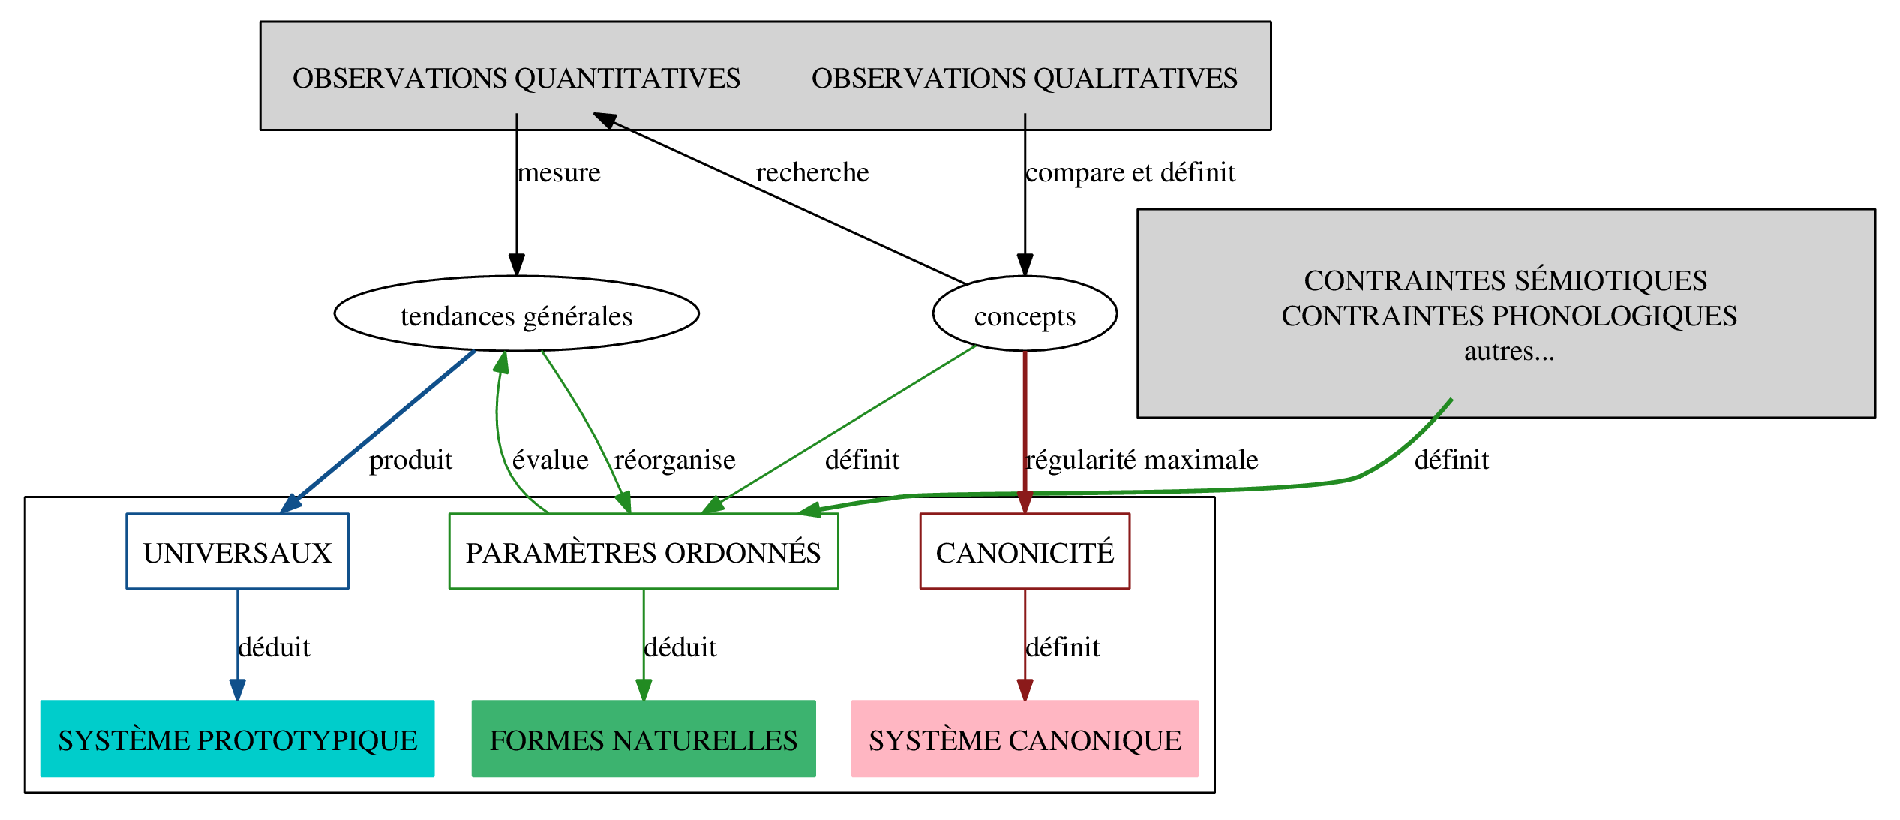
\includegraphics[width=120mm]{protonatcanon}
%\caption{Latin inflection zones}
\label{fig:canonicity}
\end{center}
\end{frame}

\begin{frame}
\frametitle{\darkhighlightiii{Comparaison de systèmes morphologiques}}
%\pause
\begin{wideitemize}
\item {Enjeux généraux en typologie linguistique}
\begin{smallwideitemize}
  \item {décrire des propriétés partagées par des systèmes}
  \item {décrire les différences entre ces systèmes}
  \item {développer le vocabulaire adéquat pour les caractériser}
\end{smallwideitemize}
%\item Canonical typology in particular
%\pause
\item {Emploi de standards comparatifs}
%\pause
\begin{smallwideitemize}
\item {Il existe plusieurs critères possibles parmi lesquels:}
\begin{smallwideitemize}
  \item {prototypes dérivables d'universaux linguistiques \cite{greenberg63}}
  \item {naturalité \cite{wurzel84,dressler00}}
  \item {canonicité \cite{corbett03,corbett07b}}
\end{smallwideitemize}
\end{smallwideitemize}
\pause
% \item \highlightii{\parsli}
% \begin{smallwideitemize}
% \item \highlightii{a formal approach to typology} w.r.t inflectional morphology.
% \item Development of measures for quantitave typological evaluation of
%   morphological systems.
% \end{smallwideitemize}
%\pause
\item Canonicité {\small --- approche autonome reposant sur un système
    d'ontologies}
\begin{smallwideitemize}
  \item la définition du canon repose sur des \lighthighlightiii{propriétés définitoires}
  \item il est défini par un \lighthighlightiii{espace multidimensionnel} des possibles
  \item il permet de comparer chaque système individuel en
    termes de \lighthighlightiii{déviation plus ou moins marquée par rapport à un
      \lighthighlightiii{étalon canonique}}
\end{smallwideitemize}
%\pause
%\item here: \highlighti{Canonical Inflection}
\end{wideitemize}
\end{frame}


\begin{frame}[t]{Représentation du canon selon Corbett {\em et al.} (2012) \nocite{corbett12imm}}
\begin{center}
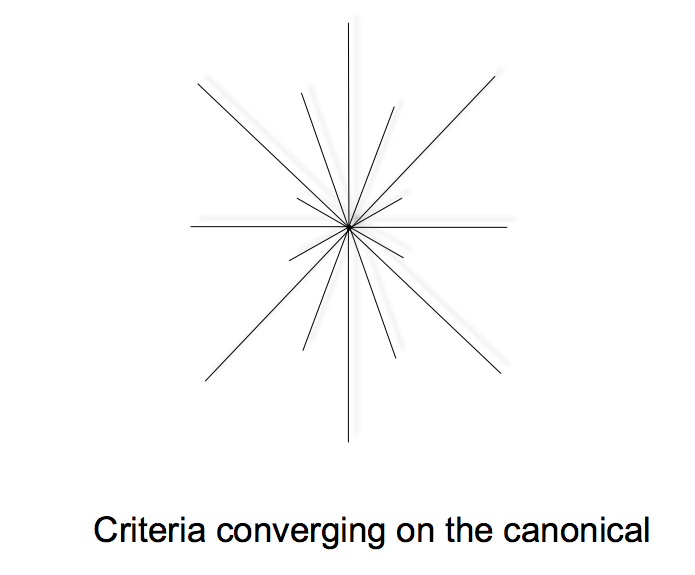
\includegraphics[width=80mm]{corbett-canon-star}
%\caption{Latin inflection zones}
\label{fig:canonicity}
\end{center}
\end{frame}


\begin{frame}
\frametitle{La typologie canonique}
\begin{wideitemize}
\item Concept de {\em typologie canonique}: \cite{corbett03}.
\item Différence entre un état hypothétique, idéal (c'est-à dire {\em
    canonique}) et les phénomènes réels qui sont observables.
\item {\em Flexion
  canonique} $\neq${\em  flexion prototypique}:
\begin{smallwideitemize}
%\item Canonical inflection is rare.
\item La flexion canonique correspond à un état idéal;
\item Elle constitue un espace théorique depuis lequel on peut mesurer
  les écarts observables,~\cite{corbett07b}.
\item Pour la comparaison entre les langues (notion typologique).
\end{smallwideitemize}
\item Quelques phénomènes non-canoniques:
\begin{smallwideitemize}
\item {\em supplétion} \cite{boye06,bonami06},
\item {\em déponence} \cite{baerman07bookdepo}, 
\item {\em hétéroclise} \cite{stump06a},
\item {\em
  défectivité} \cite{baerman10defectbook}
\item et plus récemment {\em
  surabondance} \cite{thornton10}.
\end{smallwideitemize}
\end{wideitemize}
\end{frame}

\subsection{La flexion canonique}


\begin{frame}
\frametitle{La flexion canonique}
La flexion canonique se définit par la comparaison des cases dans le
paradigme d'un lexème donné et par comparaison des paradigmes de
différents lexèmes entre eux.\\
Les cases sont censées avoir la même structure.

\scriptsize

\begin{table}
%\end{wideitemize}
\begin{tabular}{|l| p{1mm}|ll|p{1mm}|ll|p{1mm}cl}
\cline{1-1}\cline{3-4}\cline{6-7}
Traits&&\multicolumn{2}{|c|}{\textsc{ lexème~1}}&&\multicolumn{2}{|c|}{\textsc{ lexème~2}}&&\\
\cline{1-1}\cline{3-4}\cline{6-7}
\textsc{1.sg}&& radical1& {\em --ma}&&radical2& {\em
  --ma}&&\cellcolor{ciel}~~~&identique\\
\cline{1-1}\cline{3-4}\cline{6-7}
\textsc{2.sg}& &radical1&{\em --sa}&&radical2& {\em --sa}&&&\\
\cline{1-1}\cline{3-4}\cline{6-7}

\textsc{3.sg}&& radical1&{\em --ta}&&radical2& {\em
  --ta}&&\cellcolor{mandarine}&différent\\
\cline{1-1}\cline{3-4}\cline{6-7}
\textsc{1.pl}&&radical1& {\em --mo}&&radical2& {\em --mo}&&\\
\cline{1-1}\cline{3-4}\cline{6-7}
\textsc{2.pl}&&radical1& {\em --so}&&radical2& {\em --so}&&\\
\cline{1-1}\cline{3-4}\cline{6-7}
\textsc{3.pl}&&radical1& {\em --to}&&radical2& {\em --to}&&\\
\cline{1-1}\cline{3-4}\cline{6-7}
\end{tabular}\\[1mm]
\end{table}
\end{frame}

\iffalse
\begin{frame}
\frametitle{Canonical Inflection: criteria from \cite{corbett07b}}
\begin{table}\centering
\scalebox{0.88}{
\noindent\begin{tabular}{lp{4cm}@{~~~}l@{~~~}l}
\hline
&&\textsc{ comparison across }&\textsc{
  comparison }\\
&&\textsc{ cells of a lexème}&\textsc{
  across lexèmes}\\
\hline
1~~~&\textsc{ composition/structure} & {\em identique}& {\em identique}\\[1em]
2~~~&\textsc{ matériau lexical}  ($\approx$~apparence du radical) & {\em identique}& {\em différent}\\[1em]
3~~~&\textsc{ matériau flexionnel} ($\approx$~apparence des marques flex.)& {\em différent}& {\em identique}\\[1em]
4~~~&\textsc{ forme produite}  ($\approx$~apparence du mot-forme)& {\em différent}& {\em différent}\\[1em]\hline
&\\[-6pt]
\end{tabular}
}
\caption{La flexion canonique selon\cite{corbett07b}.}
\label{tbl:canonical-infl-corbett}
\end{table}
\end{frame}
\fi

\begin{frame}
\frametitle{Flexion canonique}
Comparaison des cases d'un paradigme donné.

\scriptsize

\begin{table}
%\end{wideitemize}
\begin{tabular}{|l| p{1mm}|ll|p{1mm}|ll|p{1mm}cl}
\cline{1-1}\cline{3-4}\cline{6-7}
Traits&&\multicolumn{2}{|c|}{\cellcolor{white}\textsc{ lexème~1}}&&\multicolumn{2}{|c|}{\textsc{ lexème~2}}&&\\
\cline{1-1}\cline{3-4}\cline{6-7}
\textsc{1.sg}&& \cellcolor{ciel}radical1& {\em --ma}&&radical2& {\em
  --ma}&&\cellcolor{ciel}~~~&identique\\
\cline{1-1}\cline{3-4}\cline{6-7}
\textsc{2.sg}& &radical1&{\em --sa}&&radical2& {\em --sa}&&&\\
\cline{1-1}\cline{3-4}\cline{6-7}

\textsc{3.sg}&& radical1&{\em --ta}&&radical2& {\em
  --ta}&&\cellcolor{mandarine}&différent\\
\cline{1-1}\cline{3-4}\cline{6-7}
\textsc{1.pl}&&radical1& {\em --mo}&&radical2& {\em --mo}&&\\
\cline{1-1}\cline{3-4}\cline{6-7}
\textsc{2.pl}&&radical1& {\em --so}&&radical2& {\em --so}&&\\
\cline{1-1}\cline{3-4}\cline{6-7}
\textsc{3.pl}&&radical1& {\em --to}&&radical2& {\em --to}&&\\
\cline{1-1}\cline{3-4}\cline{6-7}
\end{tabular}\\[1mm]
\end{table}
\end{frame}

\begin{frame}
\frametitle{Flexion canonique}
Comparaison des cases d'un paradigme donné.

\scriptsize

\begin{table}
%\end{wideitemize}
\begin{tabular}{|l| p{1mm}|ll|p{1mm}|ll|p{1mm}cl}
\cline{1-1}\cline{3-4}\cline{6-7}
Traits&&\multicolumn{2}{|c|}{\cellcolor{white}\textsc{ lexème~1}}&&\multicolumn{2}{|c|}{\textsc{ lexème~2}}&&\\
\cline{1-1}\cline{3-4}\cline{6-7}
\textsc{1.sg}&& \cellcolor{ciel}radical1& {\em --ma}&&radical2& {\em
  --ma}&&\cellcolor{ciel}~~~&identique\\
\cline{1-1}\cline{3-4}\cline{6-7}
\textsc{2.sg}& &\cellcolor{ciel}radical1&{\em --sa}&&radical2& {\em --sa}&&&\\
\cline{1-1}\cline{3-4}\cline{6-7}

\textsc{3.sg}&& \cellcolor{ciel}radical1&{\em --ta}&&radical2& {\em
  --ta}&&\cellcolor{mandarine}&différent\\
\cline{1-1}\cline{3-4}\cline{6-7}
\textsc{1.pl}&&\cellcolor{ciel}radical1& {\em --mo}&&radical2& {\em --mo}&&\\
\cline{1-1}\cline{3-4}\cline{6-7}
\textsc{2.pl}&&\cellcolor{ciel}radical1& {\em --so}&&radical2& {\em --so}&&\\
\cline{1-1}\cline{3-4}\cline{6-7}
\textsc{3.pl}&&\cellcolor{ciel}radical1& {\em --to}&&radical2& {\em --to}&&\\
\cline{1-1}\cline{3-4}\cline{6-7}
\end{tabular}\\[1mm]
\end{table}
\end{frame}

\begin{frame}
\frametitle{Flexion canonique}
Comparaison des cases d'un paradigme donné.

\scriptsize

\begin{table}
%\end{wideitemize}
\begin{tabular}{|l| p{1mm}|ll|p{1mm}|ll|p{1mm}cl}
\cline{1-1}\cline{3-4}\cline{6-7}
Traits&&\multicolumn{2}{|c|}{\cellcolor{white}\textsc{ lexème~1}}&&\multicolumn{2}{|c|}{\textsc{ lexème~2}}&&\\
\cline{1-1}\cline{3-4}\cline{6-7}
\textsc{1.sg}&& \cellcolor{ciel}radical1& \cellcolor{mandarine}{\em --ma}&&radical2& {\em
  --ma}&&\cellcolor{ciel}~~~&identique\\
\cline{1-1}\cline{3-4}\cline{6-7}
\textsc{2.sg}& &\cellcolor{ciel}radical1&{\em --sa}&&radical2& {\em --sa}&&&\\
\cline{1-1}\cline{3-4}\cline{6-7}

\textsc{3.sg}&& \cellcolor{ciel}radical1&{\em --ta}&&radical2& {\em
  --ta}&&\cellcolor{mandarine}&différent\\
\cline{1-1}\cline{3-4}\cline{6-7}
\textsc{1.pl}&&\cellcolor{ciel}radical1& {\em --mo}&&radical2& {\em --mo}&&\\
\cline{1-1}\cline{3-4}\cline{6-7}
\textsc{2.pl}&&\cellcolor{ciel}radical1& {\em --so}&&radical2& {\em --so}&&\\
\cline{1-1}\cline{3-4}\cline{6-7}
\textsc{3.pl}&&\cellcolor{ciel}radical1& {\em --to}&&radical2& {\em --to}&&\\
\cline{1-1}\cline{3-4}\cline{6-7}
\end{tabular}\\[1mm]
\end{table}
\end{frame}

\begin{frame}
%\frametitle{Canonical Inflection}
\frametitle{Flexion canonique}
Comparaison des cases d'un paradigme donné.

\scriptsize

\begin{table}
%\end{wideitemize}
\begin{tabular}{|l| p{1mm}|ll|p{1mm}|ll|p{1mm}cl}
\cline{1-1}\cline{3-4}\cline{6-7}
Traits&&\multicolumn{2}{|c|}{\cellcolor{white}\textsc{ lexème~1}}&&\multicolumn{2}{|c|}{\textsc{ lexème~2}}&&\\
\cline{1-1}\cline{3-4}\cline{6-7}
\textsc{1.sg}&& \cellcolor{ciel}radical1& \cellcolor{mandarine}{\em --ma}&&radical2& {\em
  --ma}&&\cellcolor{ciel}~~~&identique\\
\cline{1-1}\cline{3-4}\cline{6-7}
\textsc{2.sg}& &\cellcolor{ciel}radical1&\cellcolor{mandarine}{\em --sa}&&radical2& {\em --sa}&&&\\
\cline{1-1}\cline{3-4}\cline{6-7}

\textsc{3.sg}&& \cellcolor{ciel}radical1&\cellcolor{mandarine}{\em --ta}&&radical2& {\em
  --ta}&&\cellcolor{mandarine}&différent\\
\cline{1-1}\cline{3-4}\cline{6-7}
\textsc{1.pl}&&\cellcolor{ciel}radical1& \cellcolor{mandarine}{\em --mo}&&radical2& {\em --mo}&&\\
\cline{1-1}\cline{3-4}\cline{6-7}
\textsc{2.pl}&&\cellcolor{ciel}radical1& \cellcolor{mandarine}{\em --so}&&radical2& {\em --so}&&\\
\cline{1-1}\cline{3-4}\cline{6-7}
\textsc{3.pl}&&\cellcolor{ciel}radical1& \cellcolor{mandarine}{\em --to}&&radical2& {\em --to}&&\\
\cline{1-1}\cline{3-4}\cline{6-7}
\end{tabular}\\[1mm]
\end{table}
\end{frame}

\begin{frame}
\frametitle{Flexion canonique}
Comparaison des cases d'un paradigme à l'autre.

\scriptsize

\begin{table}
%\end{wideitemize}
\begin{tabular}{|l| p{1mm}|ll|p{1mm}|ll|p{1mm}cl}
\cline{1-1}\cline{3-4}\cline{6-7}
Traits&&\multicolumn{2}{|c|}{\cellcolor{white}\textsc{ lexème~1}}&&\multicolumn{2}{|c|}{\cellcolor{white}\textsc{ lexème~2}}&&\\
\cline{1-1}\cline{3-4}\cline{6-7}
\textsc{1.sg}&& radical1& {\em --ma}&&radical2& {\em
  --ma}&&\cellcolor{ciel}~~~&identique\\
\cline{1-1}\cline{3-4}\cline{6-7}
\textsc{2.sg}& &radical1&{\em --sa}&&radical2& {\em --sa}&&&\\
\cline{1-1}\cline{3-4}\cline{6-7}

\textsc{3.sg}&& radical1&{\em --ta}&&radical2& {\em
  --ta}&&\cellcolor{mandarine}&différent\\
\cline{1-1}\cline{3-4}\cline{6-7}
\textsc{1.pl}&&radical1& {\em --mo}&&radical2& {\em --mo}&&\\
\cline{1-1}\cline{3-4}\cline{6-7}
\textsc{2.pl}&&radical1& {\em --so}&&radical2& {\em --so}&&\\
\cline{1-1}\cline{3-4}\cline{6-7}
\textsc{3.pl}&&radical1& {\em --to}&&radical2& {\em --to}&&\\
\cline{1-1}\cline{3-4}\cline{6-7}
\end{tabular}\\[1mm]
\end{table}
\end{frame}

\begin{frame}
\frametitle{Flexion canonique}
Comparaison des cases d'un paradigme à l'autre.

\scriptsize

\begin{table}
%\end{wideitemize}
\begin{tabular}{|l| p{1mm}|ll|p{1mm}|ll|p{1mm}cl}
\cline{1-1}\cline{3-4}\cline{6-7}
Traits&&\multicolumn{2}{|c|}{\cellcolor{white}\textsc{ lexème~1}}&&\multicolumn{2}{|c|}{\cellcolor{white}\textsc{ lexème~2}}&&\\
\cline{1-1}\cline{3-4}\cline{6-7}
\textsc{1.sg}&& \cellcolor{mandarine}radical1& \cellcolor{ciel}{\em --ma}&&\cellcolor{mandarine}radical2& \cellcolor{ciel}{\em
  --ma}&&\cellcolor{ciel}~~~&identique\\
\cline{1-1}\cline{3-4}\cline{6-7}
\textsc{2.sg}& &radical1&{\em --sa}&&radical2& {\em --sa}&&&\\
\cline{1-1}\cline{3-4}\cline{6-7}

\textsc{3.sg}&& radical1&{\em --ta}&&radical2& {\em
  --ta}&&\cellcolor{mandarine}&différent\\
\cline{1-1}\cline{3-4}\cline{6-7}
\textsc{1.pl}&&radical1& {\em --mo}&&radical2& {\em --mo}&&\\
\cline{1-1}\cline{3-4}\cline{6-7}
\textsc{2.pl}&&radical1& {\em --so}&&radical2& {\em --so}&&\\
\cline{1-1}\cline{3-4}\cline{6-7}
\textsc{3.pl}&&radical1& {\em --to}&&radical2& {\em --to}&&\\
\cline{1-1}\cline{3-4}\cline{6-7}
\end{tabular}\\[1mm]
\end{table}
\end{frame}


\begin{frame}
\frametitle{Flexion canonique}
Comparaison des cases d'un paradigme à l'autre.

\scriptsize

\begin{table}
%\end{wideitemize}
\begin{tabular}{|l| p{1mm}|ll|p{1mm}|ll|p{1mm}cl}
\cline{1-1}\cline{3-4}\cline{6-7}
Traits&&\multicolumn{2}{|c|}{\cellcolor{white}\textsc{ lexème~1}}&&\multicolumn{2}{|c|}{\cellcolor{white}\textsc{ lexème~2}}&&\\
\cline{1-1}\cline{3-4}\cline{6-7}
\textsc{1.sg}&& \cellcolor{mandarine}radical1& {\em --ma}&&\cellcolor{mandarine}radical2& {\em
  --ma}&&\cellcolor{ciel}~~~&identique\\
\cline{1-1}\cline{3-4}\cline{6-7}
\textsc{2.sg}& &radical1&\cellcolor{ciel}{\em --sa}&&radical2&\cellcolor{ciel} {\em --sa}&&&\\
\cline{1-1}\cline{3-4}\cline{6-7}
\textsc{3.sg}&& radical1&{\em --ta}&&radical2& {\em
  --ta}&&\cellcolor{mandarine}&différent\\
\cline{1-1}\cline{3-4}\cline{6-7}
\textsc{1.pl}&&radical1& {\em --mo}&&radical2& {\em --mo}&&\\
\cline{1-1}\cline{3-4}\cline{6-7}
\textsc{2.pl}&&radical1& {\em --so}&&radical2& {\em --so}&&\\
\cline{1-1}\cline{3-4}\cline{6-7}
\textsc{3.pl}&&radical1& {\em --to}&&radical2& {\em --to}&&\\
\cline{1-1}\cline{3-4}\cline{6-7}
\end{tabular}\\[1mm]
\end{table}
\end{frame}


\begin{frame}
\frametitle{Flexion canonique}
Comparaison des cases d'un paradigme à l'autre.

\scriptsize

\begin{table}
%\end{wideitemize}
\begin{tabular}{|l| p{1mm}|ll|p{1mm}|ll|p{1mm}cl}
\cline{1-1}\cline{3-4}\cline{6-7}
Traits&&\multicolumn{2}{|c|}{\cellcolor{white}\textsc{ lexème~1}}&&\multicolumn{2}{|c|}{\cellcolor{white}\textsc{ lexème~2}}&&\\
\cline{1-1}\cline{3-4}\cline{6-7}
\textsc{1.sg}&& \cellcolor{mandarine}radical1& {\em --ma}&&\cellcolor{mandarine}radical2& {\em
  --ma}&&\cellcolor{ciel}~~~&identique\\
\cline{1-1}\cline{3-4}\cline{6-7}
\textsc{2.sg}& &radical1&{\em --sa}&&radical2& {\em --sa}&&&\\
\cline{1-1}\cline{3-4}\cline{6-7}

\textsc{3.sg}&& radical1&\cellcolor{ciel}{\em --ta}&&radical2& \cellcolor{ciel}{\em
  --ta}&&\cellcolor{mandarine}&différent\\
\cline{1-1}\cline{3-4}\cline{6-7}
\textsc{1.pl}&&radical1&\cellcolor{ciel}{\em --mo}&&radical2&\cellcolor{ciel}{\em --mo}&&\\
\cline{1-1}\cline{3-4}\cline{6-7}
\textsc{2.pl}&&radical1& \cellcolor{ciel}{\em --so}&&radical2&\cellcolor{ciel}{\em --so}&&\\
\cline{1-1}\cline{3-4}\cline{6-7}
\textsc{3.pl}&&radical1&\cellcolor{ciel}{\em --to}&&radical2&\cellcolor{ciel}{\em --to}&&\\
\cline{1-1}\cline{3-4}\cline{6-7}
\end{tabular}\\[1mm]
\end{table}
\end{frame}


\begin{frame}
\frametitle{Flexion canonique}
\begin{itemize}
\item toutes les formes sont différentes les unes des autres;
\item il y a exactement une forme (unique) qui exprime une structure
  de traits morphosyntaxiques donnée ($\approx$ une case= une forme phonologique/graphémique).
\end{itemize}

\scriptsize
\begin{table}
%\end{wideitemize}
\begin{tabular}{|l| p{1mm}|ll|p{1mm}|ll|p{1mm}cl}
\cline{1-1}\cline{3-4}\cline{6-7}
Traits&&\multicolumn{2}{|c|}{\cellcolor{white}\textsc{ lexème~1}}&&\multicolumn{2}{|c|}{\cellcolor{white}\textsc{ lexème~2}}&&\\
\cline{1-1}\cline{3-4}\cline{6-7}
\textsc{1.sg}&& \cellcolor{mandarine}radical1&\cellcolor{mandarine}{\em --ma}&&\cellcolor{mandarine}radical2&\cellcolor{mandarine}{\em
  --ma}&&\cellcolor{ciel}~~~&identique\\
\cline{1-1}\cline{3-4}\cline{6-7}
\textsc{2.sg}& &\cellcolor{mandarine}radical1&\cellcolor{mandarine}{\em --sa}&&\cellcolor{mandarine}radical2&\cellcolor{mandarine}{\em --sa}&&&\\
\cline{1-1}\cline{3-4}\cline{6-7}
\textsc{3.sg}&& \cellcolor{mandarine}radical1&\cellcolor{mandarine}{\em --ta}&&\cellcolor{mandarine}radical2& \cellcolor{mandarine}{\em
  --ta}&&\cellcolor{mandarine}&différent\\
\cline{1-1}\cline{3-4}\cline{6-7}
\textsc{1.pl}&&\cellcolor{mandarine}radical1&\cellcolor{mandarine}{\em --mo}&&\cellcolor{mandarine}radical2&\cellcolor{mandarine}{\em --mo}&&\\
\cline{1-1}\cline{3-4}\cline{6-7}
\textsc{2.pl}&&\cellcolor{mandarine}radical1&\cellcolor{mandarine}{\em --so}&&\cellcolor{mandarine}radical2&\cellcolor{mandarine}{\em --so}&&\\
\cline{1-1}\cline{3-4}\cline{6-7}
\textsc{3.pl}&&\cellcolor{mandarine}radical1& \cellcolor{mandarine}{\em
  --to}&&\cellcolor{mandarine}radical2&\cellcolor{mandarine}{\em --to}&&\\
\cline{1-1}\cline{3-4}\cline{6-7}
\end{tabular}\\[1mm]
\end{table}
\end{frame}


\subsection{Les phénomènes non-canoniques}

\begin{frame}
\frametitle{Phénomènes non-canoniques}
\begin{wideitemize}
\item Une fois cette régularité maximale définie, on peut définir des
  déviations pour chacune des dimensions qui la constituent
\item Méthode qui permet un typage explicite des déviations\\
\ra~ par rapport à la réalisation des formes\\
\ra~ par rapport au remplissage des
cases du paradigme\\
\ra~ dans la définition des traits morphosyntaxiques exprimés\\
\end{wideitemize}
\end{frame}


%%%%formes
\begin{frame}
\frametitle{Irrégularité dans les formes}
\framesubtitle{Syncrétismes (latin)}
\begin{center}
\begin{tabular}{l|ll|ll}
&\multicolumn{2}{c|}{\scriptsize{FILIUS}
  'fils'}&\multicolumn{2}{c}{\scriptsize{BELLUM} 'guerre'}\\
&{\scriptsize{SG}}&{\scriptsize{PL}}&{\scriptsize{SG}}&{\scriptsize{PL}}\\
\hline
{\scriptsize{NOM}}&fili-us&fili\highlightiv{-i}&bell-\highlighti{um}&bell\highlightii{-a}\\
{\scriptsize{VOC}}&fili-e&fili\highlightiv{-i}&(bell-\highlighti{um})&(bell\highlightii{-a})\\
{\scriptsize{ACC}}&fili-um&fili-\=os&bell\highlighti{-um}&bell\highlightii{-a}\\
{\scriptsize{GEN}}&fili\highlightiv{-i}&fili-\=orum&bell-i&bell-\=orum\\
{\scriptsize{DAT}}&fili\highlightiii{-\=o}&fili\highlightii{-\=is}&bell\highlightiii{-o}&bell-\highlightiv{\=is}\\
{\scriptsize{ABL}}&fili\highlightiii{-\=o}&fili\highlightii{-\=is}&bell\highlightiii{-o}&bell-\highlightiv{\=is}\\
\end{tabular}
\end{center}
\end{frame}

\begin{frame}
\frametitle{Irrégularité dans les formes}
\framesubtitle{Classes flexionnelles (latin)}
\begin{center}
\begin{tabular}{l|ll|ll}
&\multicolumn{2}{c|}{\scriptsize{FILIUS}
  'fils'}&\multicolumn{2}{c}{\scriptsize{AGRICOLA} 'paysan'}\\
&{\scriptsize{SG}}&{\scriptsize{PL}}&{\scriptsize{SG}}&{\scriptsize{PL}}\\
\hline
{\scriptsize{NOM}}&fili-us&fili\highlightiv{-i}&agricol-\highlighti{a}&agricol\highlightiii{-ae}\\
{\scriptsize{VOC}}&fili-e&fili\highlightiv{-i}&agricol-\highlighti{a}&agricol\highlightiii{-ae}\\
{\scriptsize{ACC}}&fili-um&fili-\=os&agricol{-am}&agricol{-\=as}\\
{\scriptsize{GEN}}&fili\highlightiv{-i}&fili-\=orum&agricol\highlightiii{-ae}&agricol-\=arum\\
{\scriptsize{DAT}}&fili\highlightiii{-\=o}&fili\highlightii{-\=is}&agricol\highlightiii{-ae}&agricol-\highlightiv{\=is}\\
{\scriptsize{ABL}}&fili\highlightiii{-\=o}&fili\highlightii{-\=is}&agricol-\=a&agricol-\highlightiv{\=is}\\
\end{tabular}
\end{center}
\end{frame}




\begin{frame}
\frametitle{Hétéroclise}
L'hétéroclise désigne le phénomène où le paradigme d'un lexème se
compose de parties d'au moins deux classes flexionnelles distinctes.\\[2mm]
\pause
\footnotesize
{\em Exemple: La plupart des noms d'animaux slovaques sont hétéroclites \cite{zauner73}.}\\[-2mm]
\begin{table}\small\centering
\scalebox{0.9}{
\begin{tabular}{l@{~~}|l@{~~}l@{~~}|l@{~~}l@{~~}|l@{~~}l}
\hline
&\multicolumn{2}{c@{~~~~}}{\textsc{ masc. animés}
}&
 \multicolumn{2}{c@{~~~~}}{\textsc{ 
masc. inanimés}
}
&\multicolumn{2}{c}{\textsc{ 
masc. hétéroclites}
}
\\
&\multicolumn{2}{c}{
 {\scriptsize{CHLAP}}  'gars,type'}&
 \multicolumn{2}{c}{
   {\scriptsize{DUB}}  'chêne'}
&\multicolumn{2}{c}{
 {\scriptsize{OROL}} 'aigle'}
\\
\hline
&\textsc{ singulier}&\textsc{ pluriel  }&\textsc{ singulier }&\textsc{ pluriel}&\textsc{ singulier  }&\textsc{ pluriel  }\\
\textsc{ NOM }&\cellcolor{ciel}{\em  chlap }&{\em  chlap-i}&{\em dub}&\cellcolor{mandarine}{\em dub{\bf\em -y}
}&\cellcolor{ciel}{\em orol}&\cellcolor{mandarine}{\em orl-{\bf\em y}}\\
\textsc{ GEN} &\cellcolor{ciel}{\em  chlap-a}&{\em  chlap-ov}&{\em  dub-a}&\cellcolor{mandarine}{\em dub-ov  }&\cellcolor{ciel}{\em orl-a} & \cellcolor{mandarine}{\em orl-ov}\\
\textsc{ DAT }&\cellcolor{ciel}{\em  chlap{\bf\em -ovi}}&{\em  chlap-om}&{\em
  dub-u}&\cellcolor{mandarine}{\em dub-om  }&\cellcolor{ciel}{\em orl{\bf\em -ovi}}&\cellcolor{mandarine}{\em orl-om}\\
\textsc{ ACC }&\cellcolor{ciel}{\em  chlap-a}&{\em  chlap-ov}&{\em
  dub}&\cellcolor{mandarine}{\em dub{\bf\em -y}  }&\cellcolor{ciel}{\em orl-a} & \cellcolor{mandarine}{\em orl{\bf\em -y}}\\
\textsc{ LOC} &\cellcolor{ciel}{\em  chlap{\bf\em -ovi}}&{\em  chlap-och}&{\em dub-e  }&\cellcolor{mandarine}{\em
  dub-och  }&\cellcolor{ciel}{\em orl{\bf\em -ovi}}&\cellcolor{mandarine}{\em orl-och}\\
\textsc{ INS} &\cellcolor{ciel}{\em  chlap-om}&{\em  chlap-mi}&{\em dub-om  }&\cellcolor{mandarine}{\em dub-mi  }&\cellcolor{ciel}{\em orl-om}&\cellcolor{mandarine}{\em orl-ami}\\[2ex]
\end{tabular}
}
%\caption{Heteroclisis in Slovak masculine animal names inflection}
\label{tbl:sk}
\end{table}

\end{frame}


\begin{frame}
\frametitle{Irrégularité dans les formes}
\framesubtitle{Supplétion}
\begin{description}
\item[{\bf Allomorphie}] Changement de radical, souvent conditionné phonologiquement.
\item[{\bf Supplétion de radical}] Allomorphie irrégulière extrème.
\end{description}
\end{frame}



\begin{frame}
\frametitle{Irrégularité dans les formes}
\framesubtitle{Supplétion}
\begin{wideitemize}
\item Il y a deux types de supplétion: la {\em supplétion de radical}
  et la {\em suppletion de forme} \cite{boye06}.
\item Supplétion de radical: à l'intérieur du paradigme les formes
  restent régulières et les exposants sont reconnaissables.
\item Supplétion de forme: une forme complète a été insérée dans le
  paradigme --- la forme canonique n'existe pas.
\end{wideitemize}
\end{frame}


\begin{frame}
\frametitle{Irrégularité dans les formes}
\framesubtitle{Supplétion selon \cite{boye06}}
%\pause
Supplétion de radicaux:  à l'interieur d'un paradigme; les formes à
l'intérieur d'un paradigmes sont régulières; on reconnait l'exposant.

\scriptsize
\begin{table}
\begin{tabular}{|l|p{1mm}|ll|p{1mm}|ll|p{1mm}cl}
\cline{1-1}\cline{3-4}\cline{6-7}
Traits&&\multicolumn{2}{|c|}{\scriptsize{CHANTER}}&&\multicolumn{2}{|c|}{\scriptsize{ALLER}}&&\\
\cline{1-1}\cline{3-4}\cline{6-7}
\textsc{1.sg}&& chant& {\em --e}&&v& {\em
  --ais}&&\cellcolor{ciel}~~~&régulier\\
\cline{1-1}\cline{3-4}\cline{6-7}
\textsc{2.sg} &&chant&{\em --es}&&v& {\em --as}&&&\\
\cline{1-1}\cline{3-4}\cline{6-7}
\textsc{3.sg}&& chant&{\em --e}&&v& {\em
  --a}&&\cellcolor{mandarine}&supplétif\\
\cline{1-1}\cline{3-4}\cline{6-7}
\textsc{1.pl}&&chant&\cellcolor{ciel}{\em --ons}&&\cellcolor{mandarine} all& \cellcolor{ciel}{\em --ons}&&\\
\cline{1-1}\cline{3-4}\cline{6-7}
\textsc{2.pl}&&chant& \cellcolor{ciel}{\em --ez}&&\cellcolor{mandarine} all& \cellcolor{ciel}{\em --ez}&&\\
\cline{1-1}\cline{3-4}\cline{6-7}
\textsc{3.pl}&&chant& {\em --ent}&&v& {\em --ont}&&\\
\cline{1-1}\cline{3-4}\cline{6-7}
\end{tabular}\\[1mm]
\end{table}
\end{frame}


\begin{frame}
\frametitle{Irrégularité dans les formes}
\framesubtitle{Supplétion de forme \cite{boye06}}
Supplétion de forme: une forme complète est insérée dans le paradigme
et bloque ainsi la rélisation d'autres règles.

\begin{table}
\begin{tabular}{|l| p{1mm}|ll|p{1mm}|ll|p{1mm}cl}
\cline{1-1}\cline{3-4}\cline{6-7}
Traits&&\multicolumn{2}{|c|}{\scriptsize{CHANTER}}&&\multicolumn{2}{|c|}{\scriptsize{ÊTRE}}&&\\
\cline{1-1}\cline{3-4}\cline{6-7}
\textsc{1.pl}&&chant& {\em --ons}&&\multicolumn{2}{|l|}{\cellcolor{mandarine} sommes}& {\em }&&\\
\cline{1-1}\cline{3-4}\cline{6-7}
\end{tabular}\\[1mm]
\end{table}
\end{frame}


%%%%%%%cases


\begin{frame}
\frametitle{Défectivité}
La défectivité désigne les cas où un lexème possède dans son paradigme des
cases vides (ou manquantes). 

Exemple: {\em Activa tantum} (latin) \cite{kiparsky04}: verbes de
remplacement pour combler le trou dans le sous-paradigme passif.

\noindent\eenumsentence{%\footnotesize
\item \shortex{3}{ {\scriptsize{FACIO}} & \pause $\longrightarrow$ &
    \pause  {\scriptsize{FIO}} }{``faire''&&\pause ``faire \textsc{(pass)}''}{}\pause
\item \shortex{3}{ {\scriptsize{PERDIO}}  & $\longrightarrow$ &  {\scriptsize{PEREO}}}{``détruire''&&
    ``détruire \textsc{(pass)}''}{}
}

\pause
\begin{itemize}
\item Les substituts ne
      fonctionnent pas uniquement comme formes passives de  {\scriptsize{FACIO}} 
    et {\scriptsize{PERDIO}}.
  \item Ils sont également des verbes transitifs
    indépendants à part entière.
  \item Ils constituent des entrées lexicales
    indépendantes.
\end{itemize}
\end{frame}

\begin{frame}
\frametitle{Défectivité}


\vspace{2ex}
Un autre exemple de défectivité est celui des {\em pluralia tantum}
pour lesquels il n'existe que des formes du pluriel.
\begin{itemize}
\item {\scriptsize{VIVRES}} en français,
\item {\scriptsize{TROUSERS}} 'pantalon' en anglais,
\item ou encore {\scriptsize{VIANOCE}} 'Noël' en slovaque.
\end{itemize}

\vspace{2ex}

\footnotesize
\begin{tabular}{lll}
&{\scriptsize{SG}}&{\scriptsize{PL}}\\
\hline
{\scriptsize{VIVRES}}&\cellcolor{black}&{\em vivres}\\[1ex]
{\scriptsize{TROUSERS}}&\cellcolor{black}&{\em trousers}\\[1ex]
{\scriptsize{VIANOCE}}&\cellcolor{black}&{\em Vianoce}\\[1ex]
\end{tabular}


\end{frame}




\begin{frame}
\frametitle{Surabondance}
La contre-partie évidente à la défectivité est la notion de {\em
  surabondance}. 
\begin{itemize}
\item On parle de {\em surabondance} à chaque fois qu'une
case d'un paradigme donné contient plus d'une forme.
\item La notion de
surabondance a été introduite par \cite{thornton10} pour
l'italien.
\item Deux formes: {\em cell-mates} (en), {\em compagni di cella} (it),{\em
    ``compagnons de cellule''?} (fr).
\end{itemize}

\pause
\begin{table}\centering
\scalebox{0.9}{
\begin{tabular}{l@{~~~~}l@{~~~~}l}
\hline
\textsc{ }  & \textsc{ forme~1} & \textsc{ forme~2}\\
\hline
{'languir' \textsc{ 3pl.prs.subj}}& {\em languano}& {\em languiscano}\\
[1ex]
{'posséder' \textsc{ 3pl.prs.subj}}&  {\em possiedano}& {\em posseggano}\\
[1ex]
{'posséder' \textsc{ 3sg.prs.subj}}&  {\em possieda}& {\em possegga}\\
[1ex]
{'posséder' \textsc{ 1sg.prs.subj}}&  {\em possiedo}& {\em posseggo}\\
[2ex]
\end{tabular}
}
%\caption{surabondance en \cite{thornton10}}
\label{tbl:italian}
\end{table}
\end{frame}


\begin{frame}
\frametitle{Surabondance en français}

\begin{itemize}
\item  {\em Asseoir} possède
deux formes distinctes dans la majorité de ses cases (Cf.~\cite{bonami10}).
\item Tous les verbes français en {\em
  -ayer} affichent une surabondance systématique.
\end{itemize}

\pause
\begin{table}\centering
\scalebox{0.9}{
\begin{tabular}{ccc}
    \begin{minipage}[b]{.4\linewidth}\centering\small

\scalebox{0.9}{
\begin{tabular}{l@{~~~}l@{~~~}l}
\hline
\textsc{ ind.pres}  & \textsc{ singulier} & \textsc{ pluriel}\\
\hline
\multirow{2}{*}\textsc{ p1}&  {\em assois}& {\em assoyons}\\
&  {\em assieds}& {\em asseyons}\\[1ex]
\multirow{2}{*}\textsc{ p2}& {\em assois}& {\em assoyez}\\
&  {\em assieds}& {\em asseyez}\\[1ex]
\multirow{2}{*}\textsc{ p3}&  {\em assoit}& {\em assoient}\\
&  {\em assied}& {\em asseyent}\\
\end{tabular}
}
\caption{Surabondance en français pour le verbe
  {\em asseoir}}
\label{tbl:asseoir}
\end{minipage}
&~~~~~~~~&

    \begin{minipage}[b]{.4\linewidth}\centering\small
\scalebox{0.9}{
\begin{tabular}{l@{~~~}l@{~~~}l}
\hline
\textsc{ ind.pres}  & \textsc{ singulier} & \textsc{ pluriel}\\
\hline
\multirow{2}{*}\textsc{ p1}&  {\em balaye}& \multirow{2}{*}{\em balayons}\\
&  {\em balaie}& {\em }\\[1ex]
\multirow{2}{*}\textsc{ p2}& {\em balayes}& \multirow{2}{*}{\em balayez}\\
&  {\em balaies}& {\em }\\[1ex]
\multirow{2}{*}\textsc{ p3}&  {\em balaye}& {\em balayent}\\
&  {\em balaie}& {\em balaient}\\
\end{tabular}
}
\caption{Surabondance en français pour le verbe
  {\em balayer}}
\label{tbl:balayer}
\end{minipage}
\end{tabular}
}
\end{table}
\end{frame}






%%%%%%traits

\begin{frame}
\frametitle{Décalage morphosyntaxique ou déponence}
Les noms du serbo-croate emploient parfois des formes du singulier pour
exprimer le pluriel \cite{baerman06depoData}.

\vspace{2ex}
\scalebox{0.7}{\centering
\noindent
\begin{tabular}{l@{~~}l@{~}l@{~~}l@{~}l@{~~}l@{~}l}
\hline
&
\multicolumn{2}{c}{\textsc{ 
féminin à radical en --a}
}&
\multicolumn{2}{c}{\textsc{ 
féminin à radical en --i}
}\\
&\multicolumn{2}{c}{{\scriptsize{ŽENA}} 'femme'}
&
\multicolumn{2}{c}{{\scriptsize{STVAR}} 'chose'}\\
\hline
                 &\textsc{singulier  }&\textsc{pluriel}&\textsc{singulier}&\textsc{pluriel}\\
\textsc{nom }&\cellcolor{mandarine}{\em žen-a}&{\em žen-e}&\cellcolor{ciel}{\em stvar}&{\em stvar-i}\\
\textsc{acc }&\cellcolor{mandarine}{\em žen-u} & {\em žen-e}&\cellcolor{ciel}{\em stvar}&{\em stvar-i}\\
\textsc{gen} &\cellcolor{mandarine}{\em žen-e} & {\em žen-a}&\cellcolor{ciel}{\em stvar-i}&{\em stvar-i}\\
\textsc{dat }&\cellcolor{mandarine}{\em žen-i}&{\em žen-ama}&\cellcolor{ciel}{\em stvar-i}&{\em stvar-ima}\\
\textsc{ins} &\cellcolor{mandarine}{\em žen-om}&{\em žen-ama}&\cellcolor{ciel}{\em stvar-i}&{\em stvar-im}\\[2ex]
\end{tabular}
}
\end{frame}

\begin{frame}
\frametitle{Décalage morphosyntaxique ou déponence}
Les noms du serbo-croate emploient parfois des formes du singulier pour
exprimer le pluriel \cite{baerman06depoData}.

\vspace{2ex}

\scalebox{0.7}{
\begin{tabular}{l@{~~}l@{~}l@{~~}l@{~}l}
\hline
&\multicolumn{2}{c@{~~}}{\textsc{ neut. -et$\sim$a-stem}
}&
\multicolumn{2}{c}{\textsc{ 
neut. -et$\sim$i-stem}
}\\
&\multicolumn{2}{c}{
 {\scriptsize{DETE}}  'enfant'}
&\multicolumn{2}{c}{
 {\scriptsize{TELE}}  'veau'}
\\
\hline
&\textsc{ singulier}&\textsc{ pluriel  }&\textsc{ singulier  }&\textsc{ pluriel  }\\
\textsc{ nom }& {\em  dete}& \cellcolor{mandarine}{\em dec-a}  & {\em  tele}&\cellcolor{ciel}{\em telad}\\
\textsc{ acc }& {\em  dete}& \cellcolor{mandarine}{\em dec-u} & {\em  tele}& \cellcolor{ciel}{\em telad}\\
\textsc{ gen }& {\em  deteta}& \cellcolor{mandarine}{\em dec-e} & {\em  teleta}& {\em telad}\\
\textsc{ dat }& {\em  detetu}& \cellcolor{mandarine}{\em dec-i} & {\em  teletu}& \cellcolor{ciel}{\em telad-i(ma)}\\
\textsc{ ins }& {\em  detetom  }& \cellcolor{mandarine}{\em dec-om} & {\em  teletom  }& \cellcolor{ciel}{\em telad-i(ma)  }\\[2ex]
\end{tabular}
}

\vspace{2ex}
\pause
Le fait d'employer le singulier pour
exprimer le pluriel constitue un décalage entre forme et
fonction\footnote{``A mismatch between form and
  function.''}~\cite{baerman07b}.

\end{frame}















%%%%%%%



\begin{frame}[t]{Phénomènes non-canoniques}
     \begin{columns}[t] % contents are top vertically aligned
     \begin{column}[T]{5cm} % each column can also be its own environment
\vspace*{-.5cm}
\begin{wideitemize}
\item \highlightiv{La typologie canonique en morphologie flexionnelle:}

\begin{smallwideitemize}\scriptsize
\item[\highlightii{+}] définition qualitative des différents types de déviation
  possibles par rapport au canon
\item[\highlightii{+}] notion de déviation plus ou moins importante selon les systèmes
% \end{smallwideitemize}

% % \item \highlightii{Objectif de la thèse:}

% % \begin{smallwideitemize}
% % \item[\highlightii{+}] formalisation de la définition de chaque phénomène
% % \item[\highlightii{+}] définition de mesures quantitatives
% % \end{smallwideitemize}
%  \end{wideitemize}

%      \end{column}
%      \begin{column}[T]{8cm} % alternative top-align that's better for
%                             % graphics
% %\vspace*{-4cm}
%           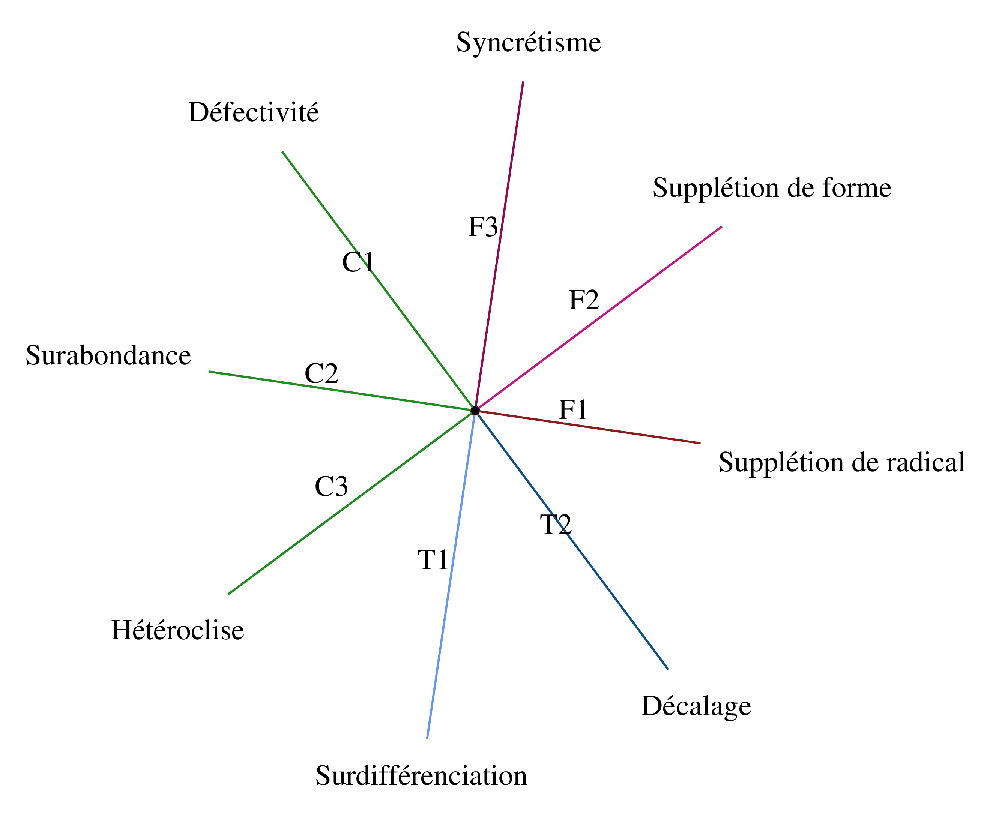
\includegraphics[height=6.5cm]{canonicity}
%      \end{column}
%      \end{columns}
% \end{frame}

% \begin{frame}[t]{Formalisation des phénomènes non-canoniques en \protect\parsli}
%      \begin{columns}[t] % contents are top vertically aligned
%      \begin{column}[T]{6cm} % each column can also be its own environment
% \vspace*{-.5cm}
% \begin{wideitemize}\footnotesize
% \item \highlightii{Formaliser la morphologie canonique:}

% \begin{smallwideitemize}\scriptsize
% \item[\highlightii{+}] définition formelle des différents types de déviation
%   possibles par rapport au canon
% \item[\highlightii{+}] raffinement de certaines définitions:\\
% \ra~allomorphie radicale/supplétion de radicaux
% \ra~défectivité/déficience
\item[\highlightii{+}] Classement possible des types de déviation:\\%\scriptsize
\ra~ dans la définition des traits: T1-T3\\
\ra~ des résultats: F1-F3\\
\ra~ dans la réalisation: C1-C4\\
\cite{walther13phd}
\end{smallwideitemize}

%\item \highlighti{Quantifier la morphologie canonique:}

% \begin{smallwideitemize}\scriptsize
% \item[\highlighti{+}] définition de mesures quantitatives des 10
%   déviations possibles par rapport au canon
% \end{smallwideitemize}

\end{wideitemize}

     \end{column}
     \begin{column}[T]{7cm} % alternative top-align that's better for
                            % graphics
%\vspace*{-4cm}
          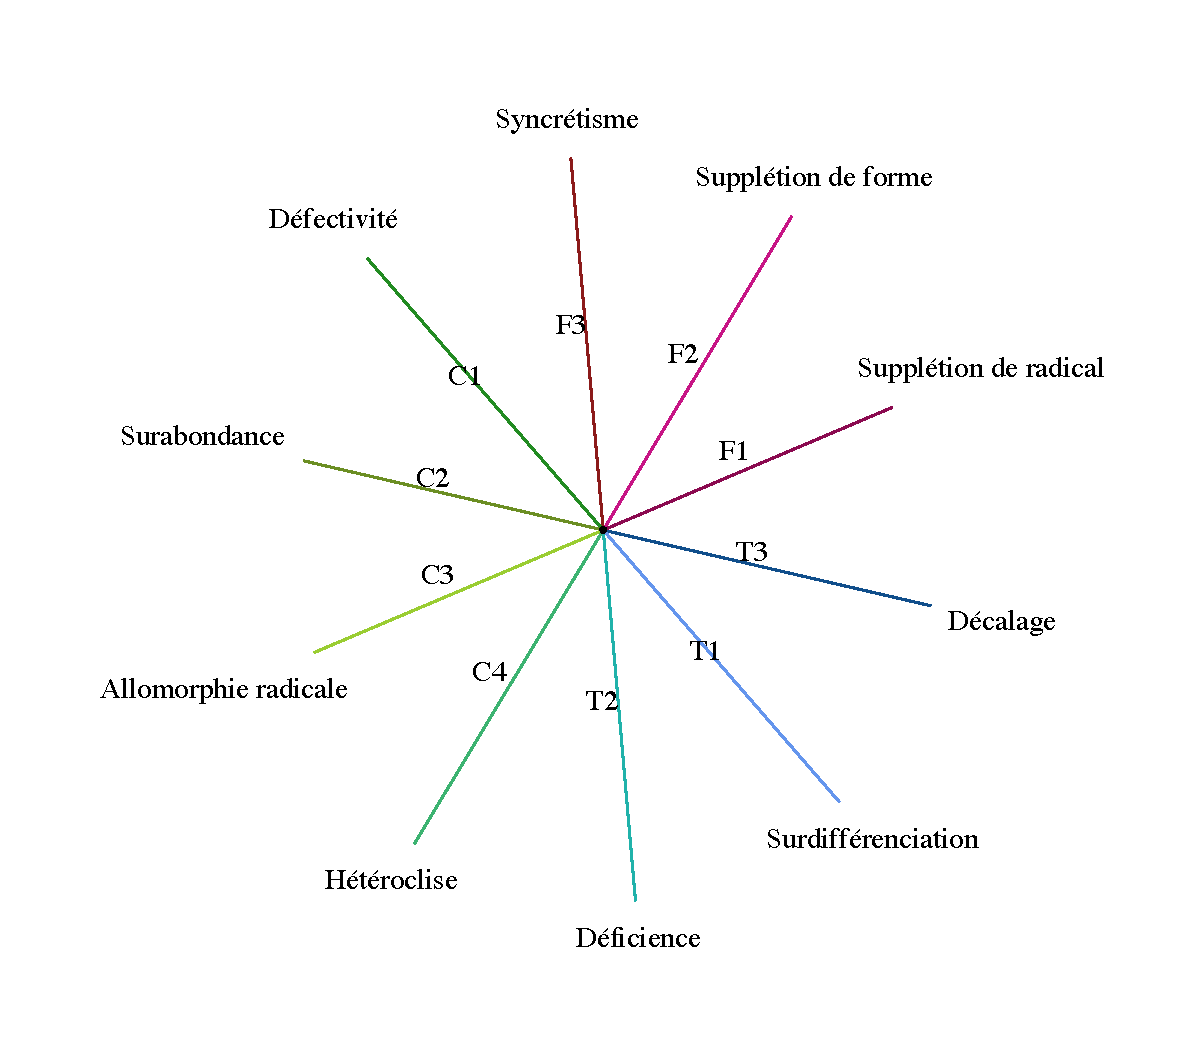
\includegraphics[height=6.4cm]{canonicityParsli}
     \end{column}
     \end{columns}

\pause
\begin{itemize}
\item[\highlighti{\danger}]\footnotesize \highlighti{Mais pas de définition pour le phénomène
  de marquage direct/inverse}
\end{itemize}
\end{frame}

\section{Une définition canonique du marquage direct/inverse}
\begin{frame}
\frametitle{Propriétés du direct/inverse (informel)}
\begin{blackwideitemize}
\item Le direct/inverse fait partie des types de marquages de
  l'alignement
\item Le plus souvent un marquage morphologique sur le verbe\\
\ra indexation des deux arguments pour les verbes transitifs
\item Identité formelle pour les formes \textsc{1sg>3sg} et
  \textsc{3sg>1sg}\\ à un \textsc{marqueur d'inverse} près
\item La présence du marquage d'inverse dépend d'une hiérarchie
  indépendante\\
\ra \textsc{hiérarchie d'agentivité/hiérarchie d'empathie} \cite[644]{delancey81}
%\pause
\end{blackwideitemize}

\ex. {\sc sap} > third person pronoun > human > animate > natural
forces > inanimate\label{ex:delancey}

\end{frame}

\begin{frame}
\frametitle{Propriétés du direct/inverse (informel)}
\begin{blackwideitemize}
\item Dans les langues du monde, les hiérarchies ne sont cependant pas
  stables \cite{jacques13inversecompass}:
\begin{smallwideitemize}
\item \textsc{1>2} et \textsc{2>1} peuvent être marqués pas des formes
  spéciales (langues algonquiennes)
\item \textsc{2>1} peut être marqué comme inverse, mais pas \textsc{1>2} (Situ Rgyalrong)
\item \textsc{1>2} et \textsc{2>1} peuvent être marqués comme inverse
  (mapuche \& langues kiranti)
\item la présence du marqueur direct ou inverse peut dépendre de
  facteurs extérieurs à la hiérarchie d'empathie (movima, japhug)
\end{smallwideitemize}
\item Cette variation est souvent analysée comme l'image d'une
  hiérarchie spécifique à ces langues
\pause
\item Autre approche: définir un standard canonique comme repère
  comparatif \highlighti{\ra régularité maximale}
\end{blackwideitemize}

\end{frame}

\begin{frame}
\frametitle{Critères de canonicité du marquage direct/inverse}
\begin{blackwideitemize}
\item Définintion de trois critères
\pause
\begin{smallwideitemize}
\item[1)] correpondance avec une hiérarchie de traits indépendante,
  maximalement régulière\\
\ra en particulier, il est toujours possible d'établir une hiérarchie
entre les arguments d'un verbe\\

\begin{center}
\ex. 1>2>{\sc 3highest}>\ldots>{\sc 3lowest}\label{ex:canhierarchy}

\end{center}

\pause
\item[2)] symmétrie diagoanale parfaite entre les cases du paradigme

\vspace*{.3cm}
\begin{tabular}{|l|llll|} 
\hline
&1 & 2 &{\sc 3h}&{\sc 3l}\\
\hline
 1 &\grise{} &1>2  & 1>{\sc 3h}&1>{\sc 3l} \\
 2&\cellcolor{infl3} 2>1 &\grise{}&2>{\sc 3h}&2>{\sc 3l}\\
 {\sc 3h}&\cellcolor{infl3} {\sc 3h}>1 &\cellcolor{infl3} {\sc 3h}>2 &\grise{}&{\sc 3h}>{\sc 3l}\\
 {\sc 3l}&\cellcolor{infl3} {\sc 3l}>1 &\cellcolor{infl3} {\sc 3l}>2 &\cellcolor{infl3} {\sc
   3l}>{\sc 3h}&\grise{}\\
\hline
%\textsc{intr}&\cellcolor[wave]{430}1&\cellcolor[wave]{530}2&\cellcolor[wave]{630}3\\
%\hline

\end{tabular}

\pause

\item[3)] autonomie par rapport à tout autre trait linguistique qui
  n'appartient pas à la hiérarchie
\end{smallwideitemize}
\end{blackwideitemize}

\begin{center}
%\ex. 1>2>{\sc 3highest}>\ldots>{\sc 3lowest}\label{ex:canhierarchy}



\end{center}
\end{frame}

\section{Les faits face au canon}
\subsection[Exemples de direct/inverse]{Quelques systèmes habituellement analysés comme relevant du direct/inverse}

% 4) Présentation de systèmes DIR/INV ± canoniques
% a) quelques systèmes de DIR/INV et leurs propriétés: zbu, khaling, dargwa, sahaptien, chuckchi (G)

\subsection[Décalages par rapport au canon]{Les exemples de systèmes à direct/inverse face au canon}
% b) étude de quelques systèmes en termes de décalage par rapport au système de DIR/INV canonique (g): 
% - décalage dans le respect de la hiérarchie: japhug - l'usage du générique (G), dargwa (g)
% - décalage dans la symétrie des cases: bantawa (même marque de DIR/INV, mais désinences par ailleurs différentes); cree (des marquages différents du DIR/INV)
% - décalage par rapport à la structuration autour de la seule hiérarchie: japhug (marquage d'une dimension discursive + l'usage du générique) (G)

\subsection[Évaluation du direct/inverse]{Évaluation canonique du statut de système à direct/inverse}
% c) évaluation de la canonicité de quelques systèmes
% i) systèmes sans DIR/INV:
% - systèmes sans marquage hiérarchique: nahuatl (G), aïnou (A)
\begin{frame}
\frametitle{Systèmes sans marquage hiérarchique}
\framesubtitle{Nahuatl}

\NoAutoSpaceBeforeFDP

\ex. ni-c-tlazohtla \\
1\textsc{sg}:A-3sg:P-aimer \\
Je l'aime.


\ex. $\varnothing$-n\=ech-tlazohtla \\
3sg:A-1\textsc{sg}:P-aimer \\
Il m'aime.

\AutoSpaceBeforeFDP

\end{frame}


% - systèmes avec marquage hiérarchique, mais sans marquage DIR/INV + hiérarchie ≠: dargwa (g)
% ii) langues clairement avec DIR/INV: zbu, khaling (une fois le DIR/INV identifié, le système se simplilfie) (g)
% iii) langues avec ± de DIR/INV: japhug, bantawa, sahaptien… (G+g — à
% discuter par Skype)


\section[Conclusion]{Conclusion and perspectives}

\begin{frame}
\frametitle{Summary and future work}
\footnotesize
\begin{wideitemize}\footnotesize
\item[\highlightii{\lefthand}]  \highlightii{Descriptive arbitrariness in morphological/linguistic analysis
  can be contained} through dedicated quantitative measures
% \begin{smallwideitemize}\footnotesize
% \item Information-theoretic methods and associated tools can provide
%   objective and reproductible ways to contrast different
%   accounts of the same data on the basis of their
%   descriptive economy
% \end{smallwideitemize}
\item[\highlightii{\lefthand}] \highlightii{Moreover compact descriptions allow for uncovering system
  internal complexity}
%\pause
\item[\highlightiv{\danger}] \highlightiv{However such measures are description-dependent}\\
\ra they require the description of data within \highlightiv{a fixed
(language-independent) linguistic model}\\
\ra measures are applied to fully \highlightiv{implemented descriptions}\\
\ra associated with \highlightiv{a large or medium scale lexicon} for ensuring a
realistic picture of the data
\begin{smallwideitemize}\footnotesize
\item In our experiment, we used the \parsli model \cite{walther13phd} and its \alexinaparsli
implementation \cite{sagot13sfcm}
\end{smallwideitemize}
\item[\highlighti{\noway}] \highlighti{This measure does not provide insight into
  cognitive complexity}
%\pause
\end{wideitemize}
% \end{frame}
% \begin{frame}
% \frametitle{Perspectives}
%\pause
\highlightii{Perspectives:}
\begin{wideitemize}\footnotesize
%\item \highlightii{Perspectives}
%\begin{smallwideitemize}\footnotesize
\item[\highlightii{\leafNE}] Extension to the \highlightii{systematic comparison of
  complexity distribution} across (related) languages 
%\end{smallwideitemize}
\end{wideitemize}
\end{frame}






\begin{frame}[t]{}
\vspace*{3cm}
\begin{center}
\Large Thank you!
\end{center}

\end{frame}

%\include{impl}
%\include{measure}
%%%%%%%
% \begin{frame} 
%  \frametitle{Références}
%  \tiny
%  \bibliographystyle{plainnat}
% \bibliography{bibliogj}
%  \end{frame}
% \end{document}


%%%%
\bibliographystyle{apalike}
%\bibliography{sfcm11}
\bibliography{these}





\end{document}

